\documentclass[a4paper]{article}
\usepackage[spanish,activeacute]{babel}
\usepackage[ansinew]{inputenc}
\usepackage{cite}
\usepackage{graphicx}
\usepackage[left=2cm,right=2cm]{geometry}
\usepackage{ulem} %Para tachar cosas
\usepackage{epigraph}
\usepackage{enumerate}
\usepackage{listings}
\usepackage{html}
\usepackage{booktabs}
\usepackage[colorlinks=true]{hyperref}
\bibliographystyle{plainurl}
\parindent = 0 pt
\parskip = 11 pt

\newcommand{\haskell}{\textsl{Haskell}}
\newcommand{\hpage}{\textbf{\textsl{$\lambda$Page}}}
\newcommand{\cabal}{\textsl{Cabal}}

\begin{document}

    \thispagestyle{empty}
    \begin{center}
	    {\Large Tesis de Licenciatura}\\[1em]
	    {\huge \textbf{$\lambda$Page}}\\[0.5em]
	    {\large \textit{Un bloc de notas para desarrolladores Haskell}}\\[1em]
	    \par\vspace{\stretch{1}}
	    {\large Departamento de Computaci\'on}\\[0.5em]
	    {\large Facultad de Ciencias Exactas y Naturales}\\[0.5em]
	    {\large Universidad de Buenos Aires}
	    \par\vspace{\stretch{1}}
	    \begin{figure}[h]
	        \begin{center}
	        
\includegraphics[width=40mm]{pictures/logoUba}
	        \end{center}
	    \end{figure}
	    {\Large \textbf{Alumno}}\\[0.8em]
	    {\Large Fernando Benavides (LU 470/01)} \par
	    {\Large greenmellon@gmail.com} \par
	    \par\vspace{\stretch{1}}
	    {\Large \textbf{Directores}}\\[0.8em]
	    {\Large Dr. Diego Garbervetsky} \par
	    {\Large Dr. Daniel Gor'in} \par
	    \par\vspace{\stretch{2}}
         {\Large \textbf{Abstract}}\\[0.5em]
    \end{center}
    El presente documento describe una herramienta para desarrolladores \haskell\ que pretende facilitar la tarea de ``debuggear'', analizar y entender c'odigo, llamada \hpage.  Con ella el usuario puede manipular ``p'aginas'' de texto libre que contengan expresiones \haskell, intentar interpretar estas expresiones independientemente y analizar los resultados obtenidos.
    \vspace*{\stretch{3}}
    \newpage

\tableofcontents

\newpage
\section{Estructura del Informe}
\paragraph{}El presente informe pretende presentar a \hpage, una herramienta para facilitar el trabajo de los desarrolladores \haskell.  El mismo se encuentra dividido en cuatro secciones.
\paragraph{}La primera es una secci'on en la que describiremos los motivos que nos llevaron a desarrollar esta herramienta, hablaremos tambi'en de otras herramientas similares y presentaremos \hpage\ de modo general, mostrando principalmente el lugar que pretendemos que ocupe dentro del mundo \haskell.
\paragraph{}En la siguiente secci'on intetaremos mostrar, a trav'es de dos tutoriales, c'omo utilizar \hpage\ y daremos a conocer sus virtudes y capacidades.  Para comenzar, aprenderemos c'omo instalarlo, de modo que el lector pueda, una vez instalado el sistema, seguir los tutoriales paso a paso y realizar sus propias experiencias.
\subparagraph{}Luego, presentaremos un tutorial destinado al p'ublico acad'emico que nos mostrar'a c'omo utilizar la herramienta para ayudar al alumno a resolver ejercicios pr'acticos t'ipicos de varias materias de la facultad.  Veremos all'i la facilidad de trabajo que brinda \hpage\ al alumno permiti'endole descubrir paso a paso el lenguaje y sus caracter'isticas principales.
\subparagraph{}El segundo tutorial que presentaremos est'a apuntado a aquellos desarrolladores que trabajan con proyectos \haskell\ de dimensiones mayores a lo visto en el 'ambito acad'emico.  La idea de este tutorial es mostrar c'omo \hpage\ puede ayudarlos a entender c'odigo existente y tambi'en a generar y testear nuevo c'odigo de manera sencilla y veloz.
\paragraph{}Una vez observado \hpage\ en funcionamiento y destacadas sus caracter'isticas principales, observaremos c'omo ha sido dise'nado y constru'ido.  Podremos ver los requerimientos que guiaron su dise'no, la arquitectura conceptual que lo subyace y las principales decisiones de dise'no e implementaci'on que se han tomado durante su desarrollo.
\paragraph{}Finalmente observaremos los resultados obtenidos y los contrastaremos con los objetivos planteados al inicio de este desarrollo.  Estableceremos el estado del proyecto en general, cu'ales son los siguientes pasos a dar y qu'e otras tareas pueden llevarse a cabo a partir de ahora.

\newpage
\section{Introducci'on}
\subsection{Motivaci'on}
\begin{epigraphs}
    \qitem{Motivation is what gets you started. Habit is what keeps you going}{Jim Rohn}
    \qitem{Essstamo mo-ti-va-do, nene}{El ``Bambino'' Veira}
\end{epigraphs}
\paragraph{}Actualmente estamos presenciando un importante cambio en el desarrollo de sistemas, gracias al 'exito de proyectos como \htmladdnormallink{CouchDB}{http://couchdb.apache.org}~\cite{couchdb}, \htmladdnormallink{ejabberd}{http://www.ejabberd.im}~\cite{ejabberd} y el chat de \htmladdnormallink{Facebook}{http://www.facebook.com/}~\cite{facebook}, todos ellos desarrollados utilizando lenguajes del paradigma funcional.
\paragraph{}Ejemplos de 'estos lenguajes de programaci'on, como \htmladdnormallink{Haskell}{http://www.haskell.org}~\cite{haskell} o \htmladdnormallink{Erlang}{http://www.erlang.org}~\cite{erlang}, demuestran ser maduros, confiables y se presentan como una alternativa a los lenguajes tradicionales del paradigma imperativo.  Sin embargo, los desarrolladores que deciden realizar el cambio de paradigma se encuentran con el problema de la escasez de ciertas herramientas que les permitan realizar su trabajo m'as eficientemente.  Por el contrario, 'estas herramientas abundan en el desarrollo de proyectos utilizando lenguajes orientados a objetos.  En particular, nuestro foco de atenci'on se centra sobre aquellas herramientas que permiten realizar \textsl{debugging} y \textsl{entendimiento} de c'odigo a trav'es de \textsl{``micro-testing''}\footnote{Enti'endase \textsl{micro-testing} como la tarea de realizar tests eventuales para entender o evaluar alg'un aspecto de un programa} .
\paragraph{}Los desarrolladores \haskell\ cuentan actualmente con las siguientes herramientas para realizar esta tarea:
\begin{description}
	\item[\htmladdnormallink{GHCi}{http://www.haskell.org/ghc/docs/latest/html/users\_guide/ghci.html}~\cite{ghci}]
		La consola que provee \htmladdnormallink{GHC}{http://www.haskell.org/ghc}~\cite{ghc} permite a los desarrolladores evaluar expresiones, verificar su tipo o su clase.  Cuenta tambi'en con un \htmladdnormallink{mecanismo de debugging}{http://www.haskell.org/ghc/docs/6.10-latest/html/users\_guide/ghci-debugger.html}~\cite{ghcdebug} integrado que permite realizar la evaluaci'on de expresiones paso a paso.  Pese a ser la herramienta m'as utilizada por los desarrolladores, \textit{GHCi} tiene varias limitaciones.  En particular:
		\begin{itemize}
			\item No permite editar m'as de una expresi'on a la vez
			\item No permite intercalar expresiones con definiciones
			\item	Si bien permite utilizar definiciones, 'estas se pierden al recargar m'odulos
			\item No es sencillo utilizar en una sesi'on las definiciones y/o expresiones creadas en sesiones anteriores
		\end{itemize}
	\item[\htmladdnormallink{Hugs}{http://www.haskell.org/hugs/}~\cite{hugs}]
		\textsl{Hugs98} es un int'erprete peque'no y port'atil de Haskell escrito en C, de modo que funciona en casi cualquier m'aquina. \textsl{Hugs98}, que se utiliza mejor como un sistema de desarrollo de programas para Haskell, se jacta de compilar extremadamente r'apido, soportar compilaci'on incremental, y tener la ventaja de un int'erprete interactivo (en el que uno puede pasar de un m'odulo a otro para probar diferentes partes de un programa).  Sin embargo, al ser un int'erprete, ni siquiera se acerca a igualar el rendimiento en tiempo de ejecuci'on de, por ejemplo, GHC.  Es, sin duda, el mejor sistema para los reci'en llegados a aprender Haskell.  Provee muchas librer'ias, inclu'idas las de Win32, un mecanismo de interfaz externa para facilitar la interoperabilidad con C y la versi'on de Windows tiene una interfaz de usuario gr'afica llamada \textsl{WinHugs}.
	\item[\htmladdnormallink{Hat}{http://www.haskell.org/hat}~\cite{hat}]
		Un herramienta para realizar seguimiento a nivel de c'odigo fuente.  A trav'es de la generaci'on de trazas de ejecuci'on, \textit{Hat} ayuda a localizar errores en los programas y es 'util para entender su funcionamiento.  Sin embargo, por estar basado en la generaci'on de trazas, requiere la compilaci'on y ejecuci'on de un programa para poder utilizarlo y esto no siempre es c'omodo para el desarrollador que puede querer simplemente analizar una expresi'on particular que incluso quiz'a no compile a'un.  Adem'as, su mantenimiento activo parece haber cesado hace m'as de un a'no y en su p'agina se observa una importante lista de problemas conocidos y caracter'isticas deseadas.
\end{description}

%%------------------------------------------------------------------------------------------------------------------------------
\subsection{Trabajos Relacionados}
\begin{epigraphs}
	\qitem{If I have seen further it is only by standing on the shoulders of giants}{Isaac Newton}
	\qitem{I like work; it fascinates me. I can sit and look at it for hours}{Jerome Klapka}
\end{epigraphs}
\paragraph{}En el mundo de la programaci'on orientada a objetos podemos encontrar herramientas como \htmladdnormallink{Java Scrapbook Pages}{http://help.eclipse.org/help33/index.jsp?topic=/org.eclipse.jdt.doc.user/reference/ref-34.htm}~\cite{javascrapbook} para \htmladdnormallink{Java}{http://www.java.com}~\cite{java} y \htmladdnormallink{Workspace}{http://wiki.squeak.org/squeak/1934}~\cite{insidesmalltalk, smalltalkworkspace} para \htmladdnormallink{SmallTalk}{http://www.smalltalk.org}~\cite{smalltalk}.  Utilizando estos aplicativos, los desarrolladores pueden introducir peque'nas porciones de c'odigo, ejecutarlas y luego inspeccionar y analizar los resultados obtenidos.  Un concepto compartido por ambas herramientas es el de presentar ``p'aginas'' de texto en las que varias expresiones pueden intercalarse con partes de texto libre y permitir al desarrollador intentar evaluar s'olo una porci'on de todo lo escrito.  Estas p'aginas pueden ser guardardas y luego recuperadas de modo de poder analizar nuevamente las mismas expresiones.  Adem'as permiten crear objetos (lo que para los lenguajes funcionales equivaldr'ia a definir expresiones) locales a la p'agina en uso y utilizarlos en ella.
\paragraph{}Dentro del paradigma funcional, con un enfoque similar, aunque un poco m'as orientado a la presentaci'on y visualizaci'on de documentos, \htmladdnormallink{Keith Hanna}{http://www.cs.kent.ac.uk/people/staff/fkh/} de la Universidad de Kent, ha desarrollado \htmladdnormallink{Vital}{http://www.cs.kent.ac.uk/projects/vital/}~\cite{vital}.  \textsl{Vital} es una implementaci'on de un entorno de visualizaci'on de documentos para \haskell.  Pretende presentar \haskell\ de una manera apropiada para usuarios finales en areas de aplicaci'on como la ingenier'ia, las matem'aticas o las finanzas.  Dentro de esta herramienta, los m'odulos \haskell\ son presentados como documentos en los que pueden visualizarse los valores que en ellos se definen directamente en el lugar en el que aparecen, ya sea de modo textual o gr'afico (como ``vistas''). 
\paragraph{}Durante el desarrollo de \hpage\ hemos tenido que enfrentar varios desaf'ios relacionados principalmente con el desarrollo de interfaces visuales dentro del paradigma funcional.  Volcando el conocimiento adquirido durante ese proceso, hemos desarrollado \htmladdnormallink{wxhNotepad}{http://github.com/elbrujohalcon/wxhnotepad}~\cite{wxhnotepad} que es, ante todo, una prueba de concepto sobre c'omo desarrollar editores de texto con \textsl{wxHaskell}.  Gracias a \htmladdnormallink{Jeremy O'Donoghue}{http://wewantarock.wordpress.com/about/}, \textsl{wxhNotepad} est'a siendo publicado como \htmladdnormallink{un tutorial}{http://wewantarock.wordpress.com/2010/01/31/building-a-text-editor-part-1/}~\cite{wewantarock} en sucesivos art'iculos en su blog
%%------------------------------------------------------------------------------------------------------------------------------
\subsection{\hpage}
\begin{epigraphs}
    \qitem{Ancorch'e lo ingegno umano faccia invenzioni varie, rispondendo con vari strumenti a un medesimo fine, mai esso trover\`a invenzione pi\`u bella, n'e pi\`u facile n'e pi\`u brieve della natura, perch'e nelle sue invenzioni nulla manca e nulla \`e superfluo}{Leonardo da Vinci}
    \qitem{La programaci'on intensiva y el uso prolongado de Tetris s'olo lleva a ver estructuras de orden y secuencias en la verduler'ia y a querer apilar los autos para formar l'ineas s'olidas}{Dar'io Ruellan}
\end{epigraphs}
\paragraph{} \htmladdnormallink{\hpage}{http://haskell.hpage.com}~\cite{hpage} se presenta como una herramienta  similar al Workspace de \textit{Smalltalk}, que permite a los desarrolladores trabajar con documentos de texto libre que incluyan expresiones y definiciones.  \hpage\ es capaz de identificar las expresiones y definiciones v'alidas y permite al desarrollador inspeccionarlas, evaluarlas, conocer su tipo y, en el caso de expresiones de tipo, conocer su g'enero (o \textsl{kind}).
\subparagraph{}En el esp'iritu de las herramientas provistas por la comunidad de desarrolladores \haskell, \hpage\ se integra con \htmladdnormallink{Cabal}{http://www.haskell.org/cabal}~\cite{cabal} y \htmladdnormallink{Hayoo!}{http://holumbus.fh-wedel.de/hayoo}~\cite{hayoo} y se encuentra ya disponible en \htmladdnormallink{HackageDB}{http://hackage.haskell.org/package/hpage}~\cite{hackage}.  \cabal\ (Common Architecture for Building Applications and Libraries) es una API distribuida con GHC que permite a un desarrollador agrupar f'acilmente un conjunto de m'odulos para producir un paquete. Es el sistema de compilaci'on est'andar para las aplicaciones y librer'ias de \haskell.  \textsl{Hayoo!} es un motor de b'usqueda especializado en la documentaci'on de la API de \haskell.  El objetivo de \textsl{Hayoo!} es proporcionar una interfaz de b'usqueda interactiva y f'acil de usar para la documentaci'on de varios paquetes y librer'ias.  Por su parte, \textsl{HackageDB} es 
un repositorio en internet de versiones de software desarrollado en \haskell, almacenadas en paquetes \cabal.
\subparagraph{}\hpage\ presenta una interfaz simple e intuitiva, desarrollada utilizando \htmladdnormallink{wxHaskell}{http://haskell.org/haskellwiki/WxHaskell}~\cite{wxhaskell}, lo que lo convierte en una aplicaci'on multiplataforma.
\subparagraph{}Por ser una herramienta desarrollada con \haskell\ para \haskell, \hpage\ se diferencia de sus pares del mundo de objetos, al aprovechar conceptos claves como son el tipado est'atico, que permite detectar errores de tipo velozmente, evitando el costo de evaluar expresiones complejas, y la evaluaci'on perezosa, que permite evaluar expresiones infinitas e ir exhibiendo resultados progresivamente.
\subparagraph{}A diferencia de \textsl{GHCi} que es una herramienta ``de consola'', \hpage\ permite visualizar resultados de manera m'as din'amica, permitiendo que errores intermedios, detectados durante la evaluaci'on de una expresi'on no impidan continuar con la misma hasta llegar a un resultado m'as completo.
\subparagraph{}\hpage\ se encuentra desarrollado utilizando \htmladdnormallink{\textsl{eprocess}}{http://hackage.haskell.org/package/eprocess}~\cite{eprocess}, una librer'ia que facilita el manejo de ``threads'' en un estilo similar al de los procesos \textsl{Erlang}.  Utilizando de esta librer'ia, \hpage\ puede realizar tareas en paralelo y por lo tanto permitir al usuario continuar editando los documentos en los que est'a trabajando mientras espera que se eval'ue una expresi'on e incluso cancelar una evaluaci'on conservando la porci'on del resultado obtenida hasta ese momento.  Por otra parte, \hpage\ utiliza \textsl{eprocess} para detectar c'alculos infinitos e informar sobre este hecho al usuario para que ya no siga esperando indefinidamente el resultado de la evaluaci'on solicitada.

\newpage
\section{Descubriendo \hpage}
\subsection{Instalaci'on}
\begin{epigraphs}
	\qitem{As a rule, software systems do not work well until they have been used, and have failed repeatedly, in real applications.}{Dave Parnas}
	\qitem{The \#1 programmer excuse for legitimately slacking off: ``My code is compiling''}{David Knutz}
\end{epigraphs}
\paragraph{}Para instalar \hpage\ en \textsl{OSX} o \textsl{Windows}, se proveen instaladores en \htmladdnormallink{el sitio web de \hpage}{http://github.com/elbrujohalcon/hPage/downloads}~\cite{hpage}, pero, como ya se ha dicho, \hpage\ se encuentra en \textsl{HackageDB} y por lo tanto el modo oficial de instalarlo es utilizando \cabal, con el siguiente comando:
\lstset{language=sh, frame=single, tabsize=2}
\begin{center}\begin{lstlisting}
$ cabal install hpage
\end{lstlisting}\end{center}
\subparagraph{}Sin embargo, para ello, previamente se deben satisfacer las siguientes dependencias:
\begin{description}
	\item[\htmladdnormallink{wxWidgets 2.8.10+}{http://www.wxwidgets.org/downloads/}~\cite{wxwidgets}] El framework de desarrollo para interfaces de usuario que utiliza \textsl{wxHaskell}.
	\item[\htmladdnormallink{Haskell Platform}{http://hackage.haskell.org/platform/}~\cite{platform}] Una distribuci'on de \haskell\ que incluye todo lo necesario para compilar e instalar programas desarrollados en este lenguaje (de particular inter'es para \hpage: \textsl{GHC} y \cabal).
\end{description}
\paragraph{}El proceso de instalaci'on de estas librer'ias y \hpage, a trav'es de \cabal\ var'ia seg'un la plataforma en la que se lo desee instalar.  Las instrucciones detalladas y actualizadas se encuentran disponibles en \htmladdnormallink{la \textsl{wiki} del sitio web de \hpage}{http://wiki.github.com/elbrujohalcon/hPage/installing-page}~\cite{hwiki}.

\newpage
\subsection{Caso de Uso: Aprobando PLP con \hpage}
\begin{epigraphs}
	\qitem{How is education supposed to make me feel smarter? Besides, every time I learn something new, it pushes some old stuff out of my brain - remember when I took that home winemaking course, and I forgot how to drive?}{Homer Simpon}
\end{epigraphs}
\paragraph{}Mostraremos a continuaci'on, a trav'es de un ejemplo, c'omo utilizar \hpage.  En este caso, hemos tomado prestada una pr'actica de la materia \textsl{Paradigmas de Lenguajes de Programaci'on}~\cite{plp}.  Exhibiremos entonces, c'omo un alumno podr'ia utilizar \hpage\ para resolver algunos de los ejercicios que all'i se presentan.  Seleccionamos s'olo aquellos que a nuestro criterio son los m'as representativos a la hora de entender c'omo \hpage\ ayuda al alumno en su resoluci'on.

\subsubsection{Pasos previos}
\paragraph{}Antes de comenzar a resolver los ejercicios, el alumno ejecuta \hpage\ y clickea en el bot'on \textsl{New}.  El programa presentar'a una pantalla similar a la de la Figura \ref{tut100}.
\begin{figure}[hp]
	\begin{center}
        	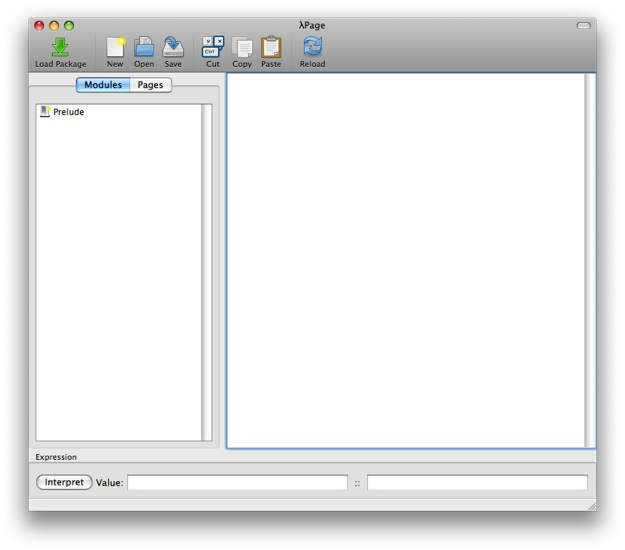
\includegraphics[width=.75\textwidth]{pictures/tut1/00}
		\caption{Tutorial 1 - Previo a comenzar}
		\label{tut100}
	\end{center}
\end{figure}

\newpage
\subsubsection{Definici'on de Tipos y Currificaci'on}
\paragraph{Ejercicio 1}Dado el siguiente programa, ?`Cu'al es el tipo de \texttt{ys}?
\lstset{language=haskell, frame=single, tabsize=4}
\begin{center}\begin{lstlisting}
	xs = [1,2,3]::[Float]
	ys = map (+) xs
\end{lstlisting}\end{center}
\subparagraph{Uso de \hpage}En el caso de este ejercicio, el alumno puede deducir que el tipo de \texttt{ys} es \texttt{[Float -> Float]}.  Para chequear su deducci'on y asegurarse de haber obtenido el resultado deseado, puede ingresar el c'odigo provisto por la c'atedra en la p'agina de \hpage, separando ambas expresiones por un rengl'on en blanco (pues ese es el modo utilizado por \hpage\ para determinar qu'e porci'on de la p'agina corresonde a cada expresi'on) y agregando la expresi'on de la que desea conocer el tipo (\texttt{ys}) al final.  Luego de ello, simplemente presiona el bot'on \textsl{Interpret} y puede observar el tipo del resultado (\texttt{[Float -> Float]}), tal como lo muestra la Figura \ref{tut101}.
\begin{figure}[hp]
	\begin{center}
        	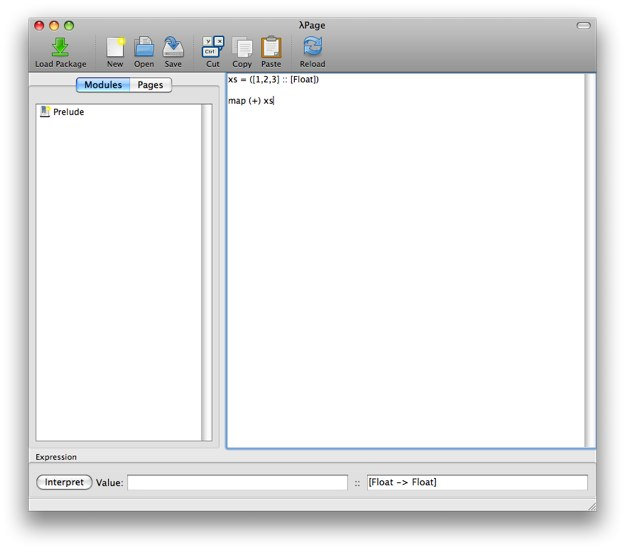
\includegraphics[width=.75\textwidth]{pictures/tut1/01}
		\caption{Tutorial 1 - Ejercicio 1}
		\label{tut101}
	\end{center}
\end{figure}

\newpage
\subsubsection{Listas por Comprensi'on}
\paragraph{Ejercicio 4}?`Cu'al es el valor de esta expresi'on?
\lstset{language=haskell, frame=single, tabsize=4}
\begin{center}\begin{lstlisting}
	[ x | x <- [1..4], y <- [x..5], (x+y) `mod` 2 == 0 ]
\end{lstlisting}\end{center}
\subparagraph{Uso de \hpage}Nuevamente, en este ejercicio el alumno puede calcular el resultado manualmente y luego utilizar \hpage\ para chequear su resultado propuesto.  Para ello, ingresa el c'odigo dentro de la p'agina, selecciona la expresi'on (pues de ese modo indica a \hpage\ que, al momento de interpretar, s'olo quiere que sea considerada esa porci'on del texto de la p'agina), y la evalu'a presionando el bot'on \textsl{Interpret}.  \hpage\ mostrar'a entonces el resultado: \texttt{[1,1,1,2,2,3,3,4]} como se ve en la Figura \ref{tut102}.
\begin{figure}[hp]
	\begin{center}
        	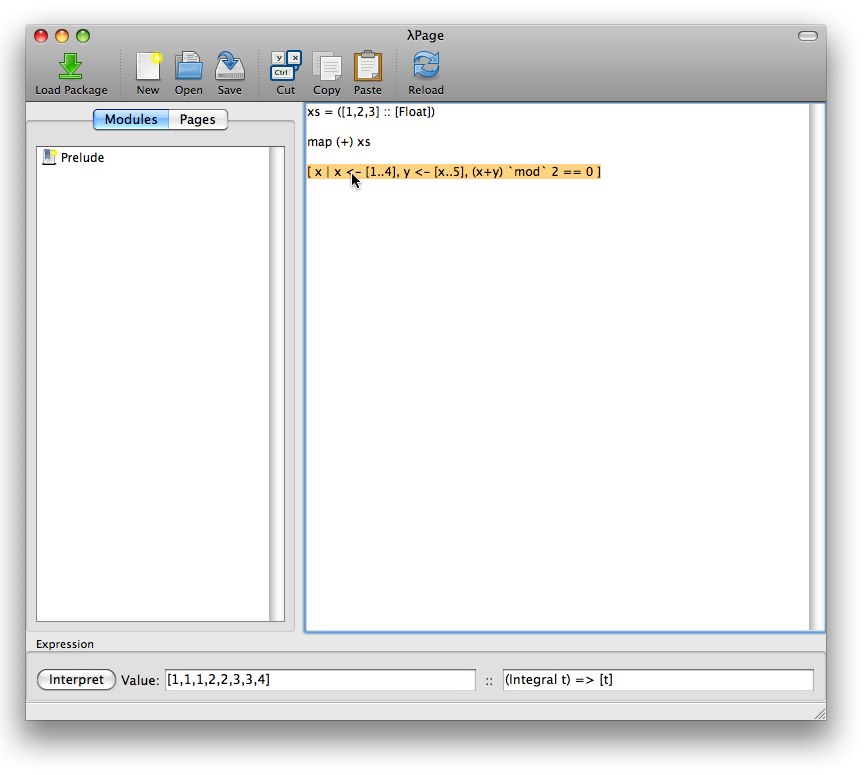
\includegraphics[width=.75\textwidth]{pictures/tut1/02}
		\caption{Tutorial 1 - Ejercicio 4}
		\label{tut102}
	\end{center}
\end{figure}

\paragraph{Ejercicio 5}Una tripla pitag'orica es una tripla $(a,b,c)$ de enteros positivos tal que $a^{2} + b^{2} = c^{2}$.  La siguiente es una definici'on de una lista (infinita) de triplas pitag'oricas.  Explicar por qu'e esta definici'on no es muy 'util.  Dar una definici'on mejor.
\begin{center}\begin{lstlisting}
pitagorica :: [(Integer,Integer,Integer)] 
pitagorica = [(a,b,c) | a <- [1..], b <-[1..], c <- [1..], a^2 + b^2 == c^2] 
\end{lstlisting}\end{center}
\subparagraph{Uso de \hpage}Para resolver este ejercicio, el alumno podr'ia comenzar por intentar evaluar la lista que se le provee, para ello reacomodar'a su definici'on tal como se observa en la Figura \ref{tut103} y, seleccionando las 'ultimas tres expresiones, presionar'a el bot'on \textsl{Interpret}.  El espacio intermedio tiene la finalidad de distinguir ambas expresiones (por un lado, la declaraci'on de tipo y, por otro, la definici'on de la expresi'on)
\begin{figure}[hp]
	\begin{center}
        	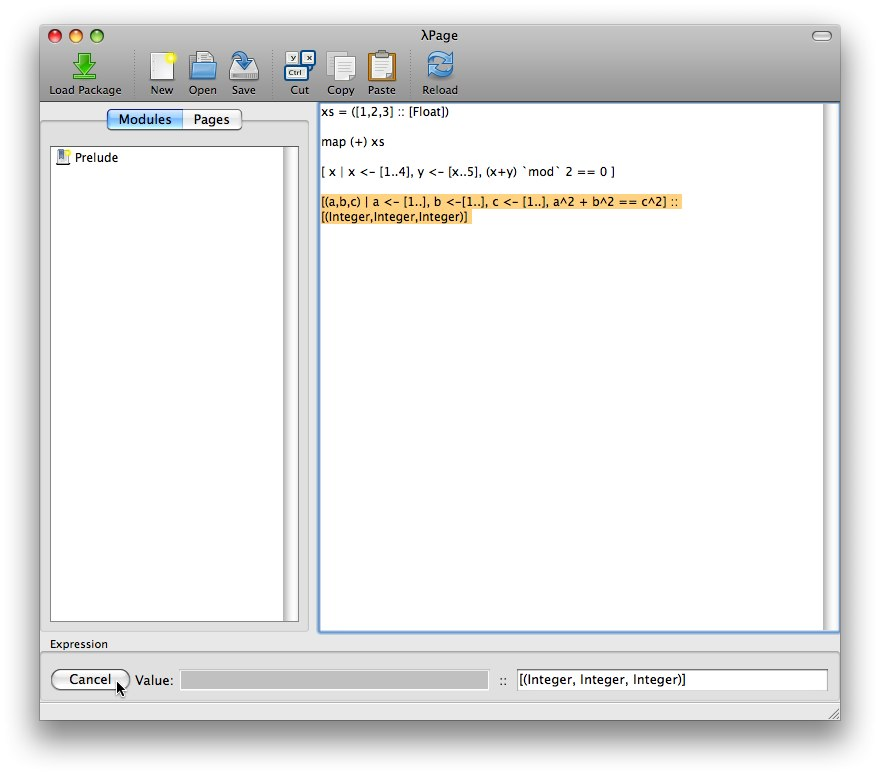
\includegraphics[width=.75\textwidth]{pictures/tut1/03}
		\caption{Tutorial 1 - Ejercicio 5 - Primer intento}
		\label{tut103}
	\end{center}
\end{figure}
\subparagraph{}El alumno podr'a observar entonces que el resultado de la interpretaci'on (si bien tiene un tipo v'alido) nunca aparece por pantalla.  Esto se debe al modo en el que se eval'uan las listas por comprensi'on en \haskell: En este caso, teniendo tres generadores (\texttt{a}, \texttt{b} y \texttt{c}) y siguiendo la sem'antica de \haskell\, para generar el primer elemento de la lista, el interprete toma el primer valor posible para \texttt{a} (o sea $1$), el primer valor posible para \texttt{b} (o sea $2$) y luego itera sobre \texttt{c}, con lo que intentar'a verificar en cada paso de esta iteraci'on que $1^{2} + 1^{2} = c$.  Pero $1^{2}+1^{2} = 2$ y sabemos que no existe ning'un n'umero natural que elevado al cuadrado sea $2$, por lo tanto, el interprete nunca encontrar'a el primer elemento de esta lista.  \hpage\ permite al alumno, pues, presionar el bot'on \textsl{Cancel} de modo de interrumpir la evaluaci'on y poder continuar trabajando.
\subparagraph{}Luego de presionar el bot'on \textsl{Cancel}, o incluso durante el lapso en el que \hpage\ trata de evaluar la expresi'on, el alumno puede modificar la definici'on de \texttt{pitagorica} para cumplir con la consigna del ejercicio.  Podr'ia, por ejemplo, reformularla como muestra la Figura \ref{tut104} e intentar interpretarla, considerando que, dentro de los n'umeros naturales se cumple que $a > c \Rightarrow a^{2} > c^{2}$ y $b > c \Rightarrow b^{2} > c^{2}$.  \hpage\ entonces, comenzar'a a exhibir resultados hasta que el alumno presione el bot'on \textsl{Cancel}.
\begin{figure}[hp]
	\begin{center}
        	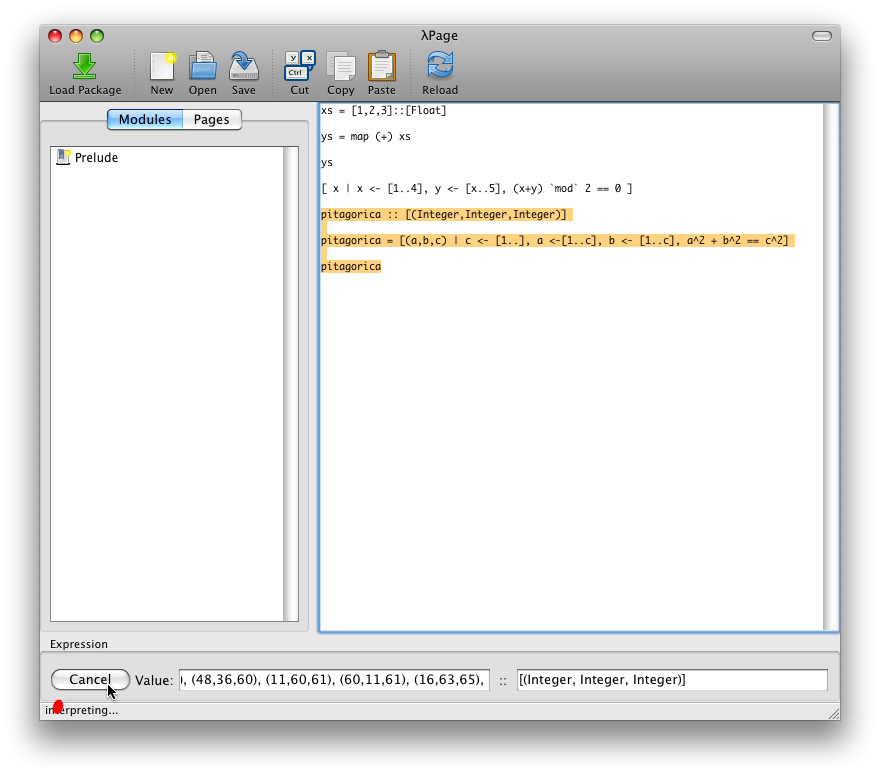
\includegraphics[width=.75\textwidth]{pictures/tut1/04}
		\caption{Tutorial 1 - Ejercicio 5 - Segundo intento}
		\label{tut104}
	\end{center}
\end{figure}
\subparagraph{}Finalmente, el alumno podr'ia tambi'en verificar que puede obtener s'olo las 5 primeras tuplas pitag'oricas, definiendo la serie pitag'orica y tomando s'olo sus primeros 5 elementos como lo muestra la Figura \ref{tut105}.  De este modo no necesitar'ia presionar el bot'on \textsl{Cancel}.
\begin{figure}[hp]
	\begin{center}
        	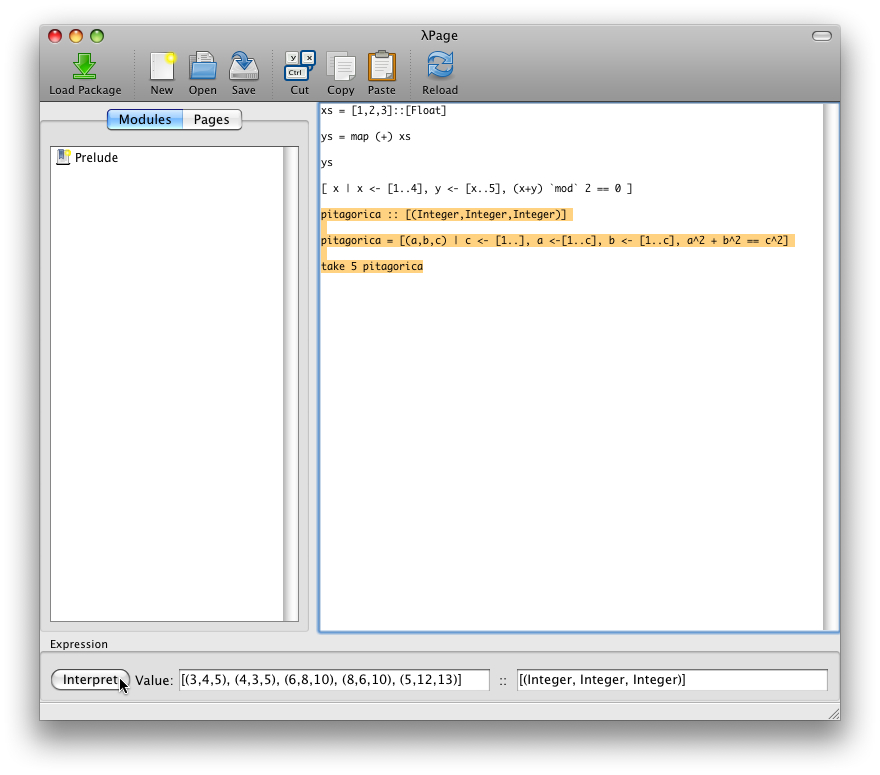
\includegraphics[width=.75\textwidth]{pictures/tut1/05}
		\caption{Tutorial 1 - Ejercicio 5 - Tercer intento}
		\label{tut105}
	\end{center}
\end{figure}

\newpage
\subsubsection{Alto Orden y Esquemas de Recursi'on}
\paragraph{Ejercicio 9}
\renewcommand{\theenumi}{\Roman{enumi}}
\begin{enumerate}
	\item Definir la funci'on \texttt{genLista}, que genera una lista de una cantidad dada de elementos, a partir de un elemento inicial y de una funci'on de incremento entre los elementos de la lista.  Dicha funci'on de incremento, dado un elemento de la lista, devuelve el elemento siguiente.
	\item Usando \texttt{genLista}, definir la funci'on \texttt{dh}, que dado un par de n'umeros (el primero menor que el segundo), devuelve una lista de n'umeros consecutivos desde el primero hasta el segundo.
\end{enumerate}
\renewcommand{\theenumi}{\arabic{enumi}}
\subparagraph{Uso de \hpage}En este caso, ciertamente \hpage\ no puede ayudar al alumno a \textsl{crear} las funciones que se le solicitan, pero s'i puede ayudarlo a testearlas.  Supongamos pues que el alumno crea una nueva p'agina y define en ella las funciones \texttt{genLista} y \texttt{dh} tal como se ve en la Figura \ref{tut106}.  Luego, intenta testear su ejercicio y, tal como se ve en la Figura \ref{tut107}, puede comprobar que sus funciones generan una recursi'on infinita.  Observa entonces que a \texttt{genLista} le falta un \textbf{caso base} y lo agrega, para luego volver a testear sus funciones como se ve en la Figura \ref{tut108} y obtener as'i el resultado esperado.  Al igual que ya hemos visto en varios casos anteriores, debe dejar un rengl'on intermedio en blanco para que \hpage\ distinga las dos partes de la definici'on de la funci'on.
\begin{figure}[hp]
	\begin{center}
        	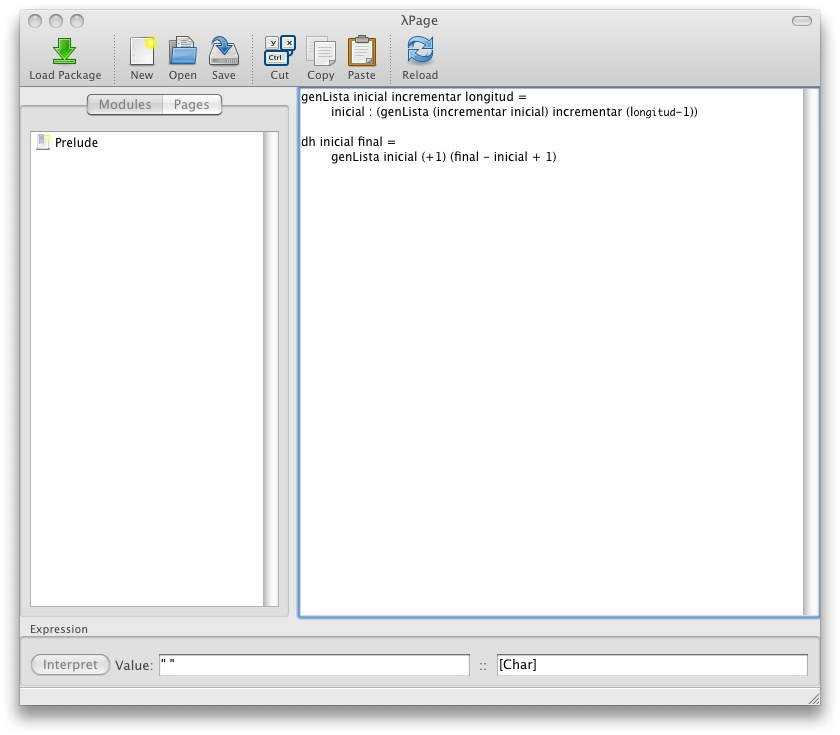
\includegraphics[width=.75\textwidth]{pictures/tut1/06}
		\caption{Tutorial 1 - Ejercicio 9 - Primer Intento}
		\label{tut106}
	\end{center}
\end{figure}
\begin{figure}[hp]
	\begin{center}
        	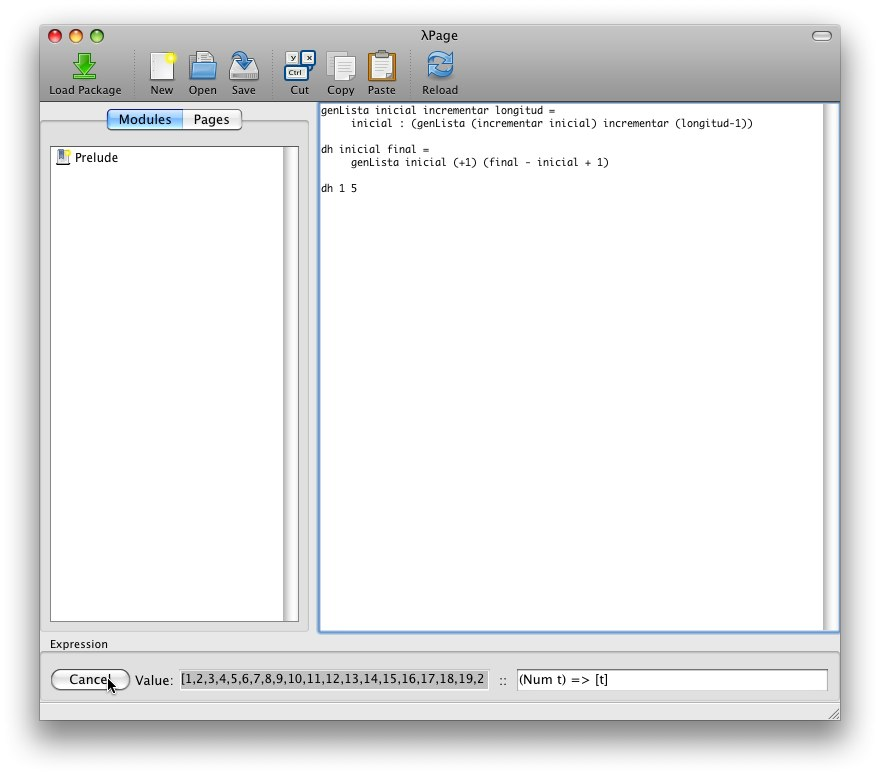
\includegraphics[width=.75\textwidth]{pictures/tut1/07}
		\caption{Tutorial 1 - Ejercicio 9 - Recursi'on Infinita}
		\label{tut107}
	\end{center}
\end{figure}
\begin{figure}[hp]
	\begin{center}
        	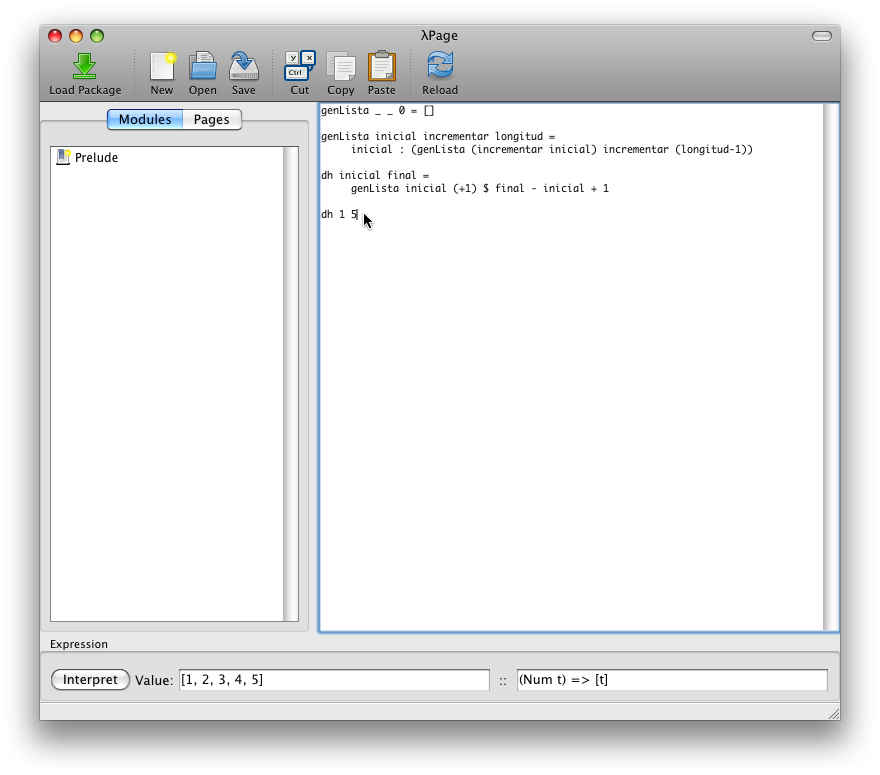
\includegraphics[width=.75\textwidth]{pictures/tut1/08}
		\caption{Tutorial 1 - Ejercicio 9 - Segundo Intento}
		\label{tut108}
	\end{center}
\end{figure}
\subparagraph{}Cabe aclarar que lo hecho en este ejercicio no es (ni pretende tampoco) ser un completo test de las funciones creadas.  Es simplemente lo que hemos llamado \textsl{micro-testing}: El ejercicio de realizar peque'nas pruebas ``a mano'' utilizando expresiones cuyo resultado de evaluaci'on es previsible.

\newpage
\paragraph{Ejercicio 23}Definimos el siguiente tipo:
\begin{center}\begin{lstlisting}
	data Agenda p t = Vacia | Telefonos p [t] (Agenda p t)
\end{lstlisting}\end{center}
\subparagraph{}Este tipo modela una agenda de tel'efonos.  A una agenda se le puede agregar una nueva entrada, donde se registra para una persona una lista de tel'efonos.  Una misma persona puede aparecer en varias entradas.  La lista de tel'efonos de una entrada puede contener repetidos.  Ejemplo:
\begin{center}\begin{lstlisting}
miAgenda = Telefonos "Letincho" [42079999,43834567] 
           (Telefonos "Javi" [47779830] (Telefonos "Letincho" [42079999] Vacia)) 
\end{lstlisting}\end{center}
\ldots
\subparagraph{Uso de \hpage}El ejercicio contin'ua, pero en este caso, el alumno podr'ia verse tentado a intentar evaluar \texttt{miAgenda} directamente en \hpage\ y obtendr'ia el resultado de la Figura \ref{tut109}.  'Esto se debe a que \hpage\ no soporta definiciones de tipos de datos directamente en el texto.  Cabe aclarar que el error obtenido no es ``prolijo'' pues viene directamente de \textsl{GHC}, cuya API (utilizada por \hpage\ a trav'es de \textsl{hint} como se ver'a en la Secci'on \ref{secImplement}) no provee errores tipados, sino s'olamente descritos en forma de texto.
\begin{figure}[hp]
	\begin{center}
        	
\includegraphics[width=.75\textwidth]{pictures/tut1/09}
		\caption{Tutorial 1 - Ejercicio 23 - Primer Intento}
		\label{tut109}
	\end{center}
\end{figure}
\subparagraph{}Para conseguir el efecto deseado, el alumno puede crear un m'odulo (sin salir de \hpage) y guardarlo utilizando la opci'on \textsl{Page $\rightarrow$ Save As\ldots} o el bot'on \textsl{Save}) tal como se observa en la Figura \ref{tut110}.  Luego, utilizando la opci'on \textsl{Haskell $\rightarrow$ Load Modules\ldots} puede cargar el m'odulo reci'en creado, seleccionar la expresi'on \texttt{miAgenda} y evaluarla normalmente.  Observamos el resultado de esta operaci'on en la Figura \ref{tut111}
\begin{figure}[hp]
	\begin{center}
        	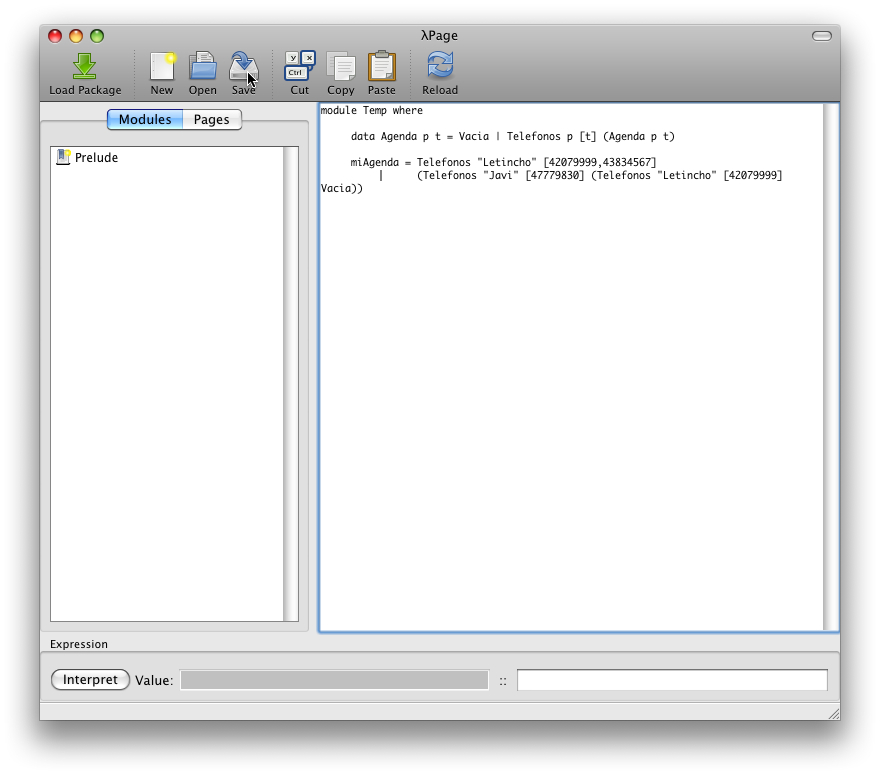
\includegraphics[width=.75\textwidth]{pictures/tut1/10}
		\caption{Tutorial 1 - Ejercicio 23 - Crear M'odulo}
		\label{tut110}
	\end{center}
\end{figure}
\begin{figure}[hp]
	\begin{center}
        	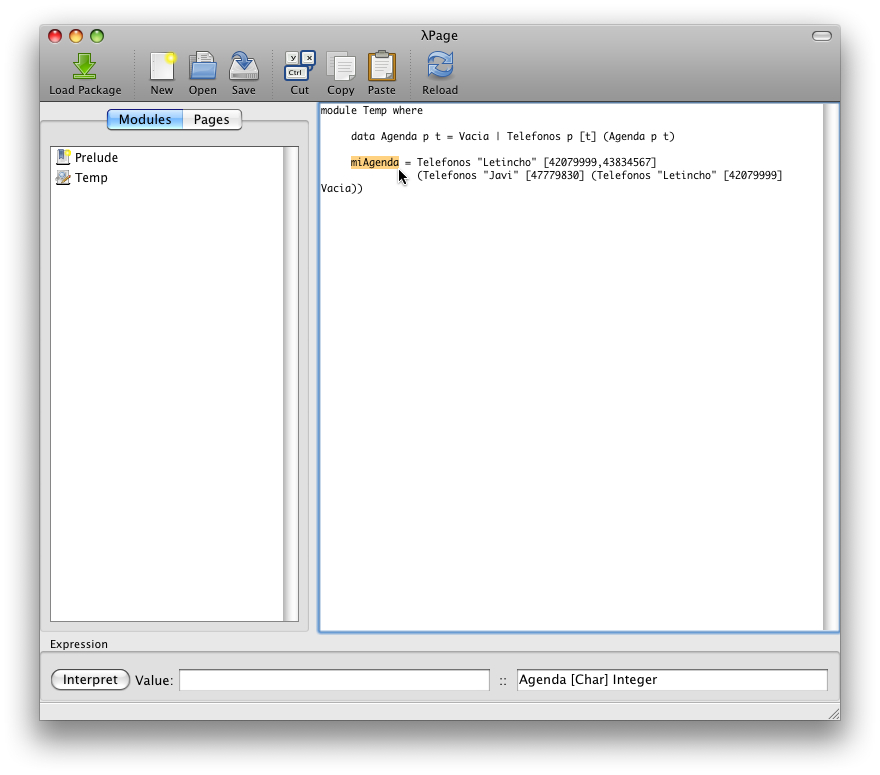
\includegraphics[width=.75\textwidth]{pictures/tut1/11}
		\caption{Tutorial 1 - Ejercicio 23 - Segundo Intento}
		\label{tut111}
	\end{center}
\end{figure}
\subparagraph{}Podemos ver, por un lado, que el resultado no ha sido mostrado, sino que s'olo se inform'o su tipo.  Esto se debe a que el tipo \texttt{Agenda} no es instancia de la clase \texttt{Show}.  Para visualizar el resultado, el alumno podr'ia agregar la cl'ausla \texttt{deriving (Show)} al tipo \texttt{Agenda}, grabar el m'odulo modificado, presionar el bot'on \textsl{Reload} y luego evaluar nuevamente \texttt{miAgenda} tal como se ve en la Figura \ref{tut112}.
\begin{figure}[hp]
	\begin{center}
        	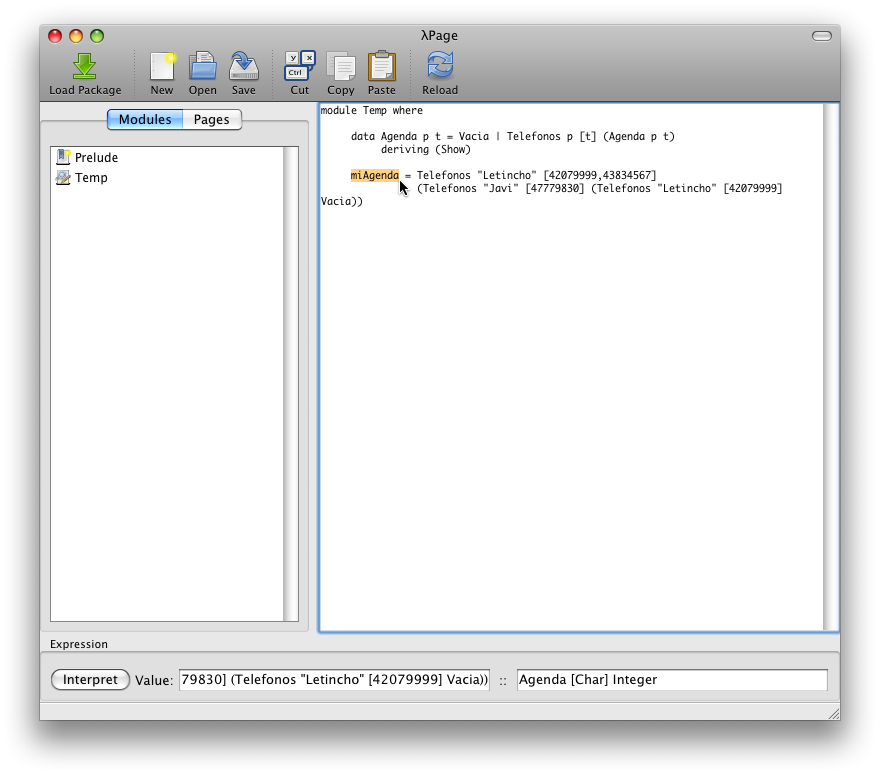
\includegraphics[width=.75\textwidth]{pictures/tut1/12}
		\caption{Tutorial 1 - Ejercicio 23 - Tercer Intento}
		\label{tut112}
	\end{center}
\end{figure}
\subparagraph{}Por otra parte, aprovecharemos este ejercicio simple para mostrar lo que \hpage\ permite hacer con los elementos de la lista \textsl{Modules}.  Presionando bot'on derecho del mouse sobre un 'item, \hpage\ despliega un men'u contextual que nos permite, entre otras opciones ``navegar''  el m'odulo y observar los elementos que exporta.  La Figura \ref{tut113} nos muestra el ``'arbol'' que se desprende de nuestro m'odulo \texttt{Temp}
\begin{figure}[hp]
	\begin{center}
        	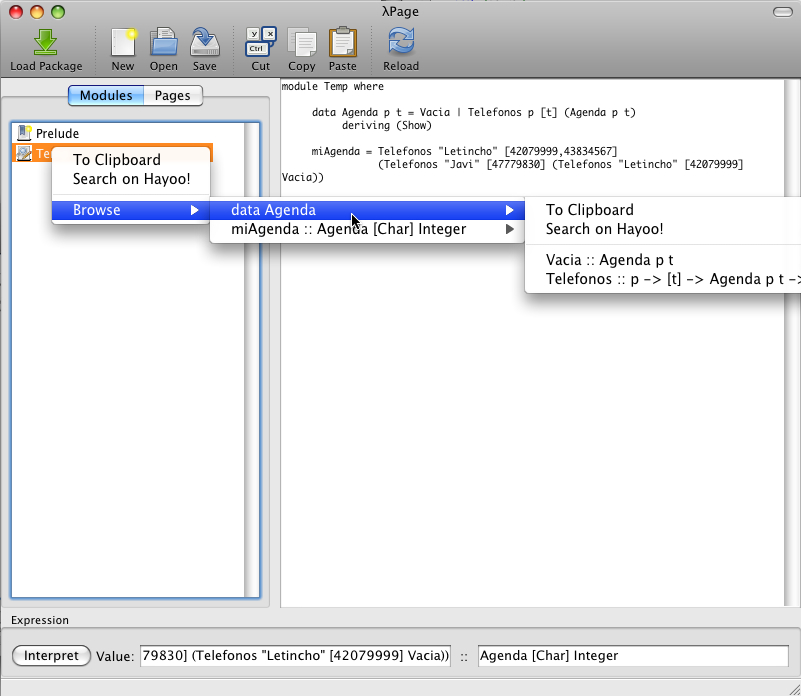
\includegraphics[width=.75\textwidth]{pictures/tut1/13}
		\caption{Tutorial 1 - Navegando M'odulos}
		\label{tut113}
	\end{center}
\end{figure}

\newpage
\subsubsection{Conclusiones}
\paragraph{}En este tutorial hemos demostrado un uso sencillo de \hpage\ como herramienta de \textsl{micro-testing}, permitiendo al usuario trabajar con las funciones definidas en el \texttt{Prelude} de \haskell\ adem'as de las que 'el mismo desee definir localmente.
\paragraph{}Pudimos apreciar c'omo \hpage\ permite definir expresiones y funciones, para luego evaluarlas de manera individual o combinada.  Pudimos ver que \hpage\ distingue unas expresiones de otras por encontrase separadas utilizando renglones en blanco.  Vimos tambi'en c'omo var'ia el contexto de interpretaci'on (o sea, las expresiones que \hpage\ toma en consideraci'on al momento de realizar una interpretaci'on):
\begin{itemize}
	\item Si el usuario seleccion'o una porci'on de texto, \hpage\ s'olo toma en consideraci'on las definiciones que se encuentren en la selecci'on e interpreta la 'ultima expresi'on del texto seleccionado
	\item Si el usuario, en cambio, no ha seleccionado texto alguno, \hpage\ toma en consideraci'on todas las definiciones de la p'agina e interpreta la expresi'on sobre la que se encuentra posicionado por el cursor
\end{itemize}
\subparagraph{}Dichas evaluaciones pueden generar diversos resultados y hemos visto c'omo se maneja \hpage\ con algunos de ellos:
\begin{itemize}
	\item Para aquellas expresiones cuyo valor no puede ser expresado en forma de texto, hemos visto c'omo \hpage\ nos permite conocer su tipo.
	\item En el caso de expresiones cuyo valor es de longitud infinita, \hpage\ exhibe todo lo que el usuario desee del resultado, culminando cuando 'este presiona el bot'on \textsl{Cancel}.
	\item Y en relaci'on a aquellas que requieren un c'alculo infinito para determinar su valor, \hpage\ muestra su tipo y permite al usuario continuar trabajando con las dem'as expresiones hasta que decida presionar el bot'on \textsl{Cancel} e interrumpir de esa manera el c'alculo.
\end{itemize}
\paragraph{}Esta forma de trabajar con los resultados, combinada con la posibilidad que brinda \hpage\ de editar definiciones de manera simple y directa, para luego volver a evaluar expresiones que las usan, permite al usuario trabajar fluidamente y le da la libertad de \textsl{cometer errores}, detectarlos, corregirlos y luego continuar su trabajo.  Esta caracter'istica de \hpage\ es muy importante sobre todo para quienes se encuentran dando sus primeros pasos en el mundo de \haskell\ pues, entendemos, facilita el aprendizaje del lenguaje.
\paragraph{}Tambi'en hemos visto en este tutorial c'omo se puede utilizar \hpage\ para crear, cargar, modificar y recargar m'odulos, trabajando siempre en una 'unica p'agina de texto.  'Esta es otra caracter'istica de \hpage\ que facilita el trabajo ya no s'olamente a los estudiantes sino a todo tipo de desarrolladores \haskell.

\newpage
\subsection{Caso de Uso: Ganando al 4 en L'inea con \hpage}
\begin{epigraphs}
	\qitem{We learn by example and by direct experience because there are real limits to the adequacy of verbal instruction}{Malcom Gladwell}
	\qitem{Look behind you, a Three-Headed Monkey!}{Guybrush Threepwood}
\end{epigraphs}
\paragraph{}Inclu'imos en este informe un segundo tutorial, apuntando esta vez a mostrar c'omo \hpage\ puede ser de utilidad para un programador \haskell\ que se enfrenta a un problema complejo.  En 'el veremos como \hpage\ ayuda al usuario a ``entender'' c'odigo escrito por otra persona (o quiz'a por el mismo, alg'un tiempo atr'as).
\subsubsection{Introducci'on}
\paragraph{}La historia comienza cuando nuestra amiga desarrolladora, a quien llamaremos \textsl{F'atima}\footnote{El nombre lo hemos elegido en honor a quien, hace ya casi 15 a'nos y utilizando el sobrenombre \textsl{Pers'efone}, fue la \textsl{maestra} y principal rival de 4 en L'inea de Fernando Benavides en \htmladdnormallink{CyberJuegos}{http://www.cyberjuegos.com}} para darle un poco de personalidad, se encuentra con la misi'on de modificar una implementaci'on de un juego de \textsl{4 en L'inea}, llamada \htmladdnormallink{hfiar}{http://hackage.haskell.org/package/hfiar}~\cite{hfiar}.  F'atima tiene que adaptar el juego de modo que permita \textsl{jugar contra la computadora} pues actualmente s'olo permite jugar a dos seres humanos entre s'i.
\subparagraph{}Como es de suponer, F'atima no conoce al creador del juego y no puede contactarlo por lo que sus 'unicas herramientas, m'as all'a de su conocimiento de \haskell\ y del juego en s'i, son el c'odigo fuente de \textsl{hfiar} y \hpage.

\subsubsection{Primeros Pasos}
\paragraph{}Para comenzar, F'atima descarga el c'odigo del programa desde \textsl{HackageDB} y lo descomprime o bien clona el repositorio \textsl{Git} con el siguiente comando:
\lstset{language=sh, frame=single, tabsize=2}
\begin{center}\begin{lstlisting}
$ git clone git://github.com/elbrujohalcon/hfiar.git
\end{lstlisting}\end{center}
\begin{figure}[hp]
	\begin{center}
        	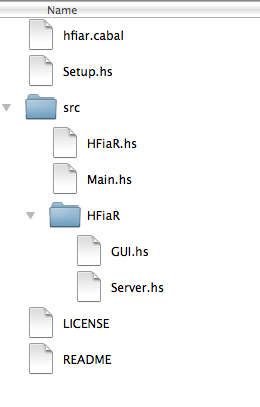
\includegraphics{pictures/tut2/00}
		\caption{Tutorial 2 - Archivos Originales}
		\label{tut200}
	\end{center}
\end{figure}
\paragraph{}Una vez hecho eso, puede observar la estructura del proyecto, tal como se ve en la Figura \ref{tut200}.  Conociendo la estructura b'asica de los proyectos desarrollados en \haskell, podemos describir los archivos all'i presentes de la siguiente manera:
\begin{description}
\item[hfiar.cabal] Archivo de descripci'on de proyecto \cabal.  F'atima puede obtener de 'el informaci'on general del proyecto, sus m'odulos, las dependencias y extensiones del lenguaje que se necesitan para compilarlo y dem'as.  
\item[Setup.hs] Archivo \haskell\ utilizado por \cabal\ para realizar tareas especiales al momento de configurar, compilar o instalar la aplicaci'on.  Junto con \textbf{hfiar.cabal} permite instalar el proyecto utilizando las siguientes instrucciones:
		\begin{center}\begin{lstlisting}
$ cabal configure --user
$ cabal build
$ cabal install
		\end{lstlisting}\end{center}
\item[src] Carpeta que contiene los archivos de c'odigo fuente del proyecto.  F'atima deber'a analizar cada uno de ellos por separado para poder comprender su funcionamiento.
\item[LICENSE] Archivo con la licencia del proyecto, en este caso \htmladdnormallink{BSD3}{http://www.linfo.org/bsdlicense.html}~\cite{bsd}.
\item[README] En el caso de este proyecto, no se trata de algo demasiado 'util, dice simplemente:
\begin{verbatim}
Four in a Row in Haskell!!
See http://hackage.haskell.org/package/hfiar
\end{verbatim}
\end{description}

\newpage
\subsubsection{Entendiendo el Proyecto}
\paragraph{}Para comenzar a entender c'omo est'a estructurada la aplicaci'on, F'atima observa el archivo \textbf{hfiar.cabal} (al que podemos ver en la Figura \ref{tut201}) y observa que el proyecto se encuentra compuesto por una librer'ia (que incluye s'olamente al m'odulo \texttt{HFiaR}) y un ejecutable llamado \texttt{hfiar} que, m'as all'a del m'odulo \texttt{Main}, incluye a los m'odulos \texttt{HFiaR.GUI} y \texttt{HFiaR.Server}.  F'atima puede ver adem'as que, para compilar los m'odulos del proyecto, debe utilizar las extensiones \textbf{MultiParamTypeClasses} y \textbf{GeneralizedNewtypeDeriving}.
\begin{figure}[hp]
	\begin{center}
	\hbox{}
		\begin{center}\begin{lstlisting}
name: hfiar
version: 2.0.4
cabal-version: >=1.6
build-type: Custom
license: BSD3
license-file: LICENSE
copyright: 2010 Fernando "Brujo" Benavides
maintainer: greenmellon@gmail.com
stability: stable
homepage: http://github.com/elbrujohalcon/hfiar
package-url: http://code.haskell.org/hfiar
bug-reports: http://github.com/elbrujohalcon/hfiar/issues
synopsis: Four in a Row in Haskell!!
description: The classical game, implemented with wxHaskell
category: Game
author: Fernando "Brujo" Benavides
tested-with: GHC ==6.12.1
data-files: LICENSE README
data-dir: ""
extra-source-files: Setup.hs
extra-tmp-files:

source-repository head
    type:     git
    location: git://github.com/elbrujohalcon/hfiar.git

Library
    build-depends: base >= 4,                   base < 5,
                   mtl >=1.1.0,                 mtl < 1.2,
                   eprocess >= 1.1.2,           eprocess < 2
    extensions: MultiParamTypeClasses, GeneralizedNewtypeDeriving
    exposed-modules: HFiaR
    hs-source-dirs: src

Executable hfiar
    build-depends: wxcore >=0.12.1.4,           wxcore < 0.13,
                   wx >=0.12.1.4,               wx < 0.13
    extensions: MultiParamTypeClasses, GeneralizedNewtypeDeriving
    main-is: Main.hs
    buildable: True
    hs-source-dirs: src
    other-modules: HFiaR.GUI, HFiaR.Server
    ghc-options: -Wall
    			\end{lstlisting}\end{center}
		\caption{Tutorial 2 - hfiar.cabal}
		\label{tut201}
	\end{center}
\end{figure}
\subparagraph{}Habiendo realizado este an'alisis, F'atima configura el proyecto ejecutando la siguiente instrucci'on:
\begin{center}\begin{lstlisting}
$ cabal configure --user
\end{lstlisting}\end{center}
\subparagraph{}Sabiendo que existe una librer'ia en el proyecto, F'atima intenta generar su documentaci'on, ejecutando:
\begin{center}\begin{lstlisting}
$ cabal haddock
\end{lstlisting}\end{center}
\subparagraph{}En el caso de \textsl{hfiar}, ese comando genera la documentaci'on en formato HTML, siendo su p'agina principal \texttt{dist/doc/html/hfiar/index.html}.  F'atima encuentra all'i una descripci'on de los componentes del m'odulo \texttt{HFiaR}.  Armada con estos datos, se dispone a utilizar \hpage\ para comprender c'omo funcionan esos componentes.

\newpage
\subsubsection{Utilizando \hpage}
\paragraph{}Una vez abierto \hpage, F'atima puede intentar cargar el proyecto utilizando la opci'on \textsl{Haskell $\rightarrow$ Load Package\ldots} o el bot'on \textsl{Load Package}.  Eso abre una ventana en la que F'atima debe seleccionar el archivo \textbf{setup-config} generado por \cabal, tal como se ve en la Figura \ref{tut202}.
\begin{figure}[hp]
	\begin{center}
        	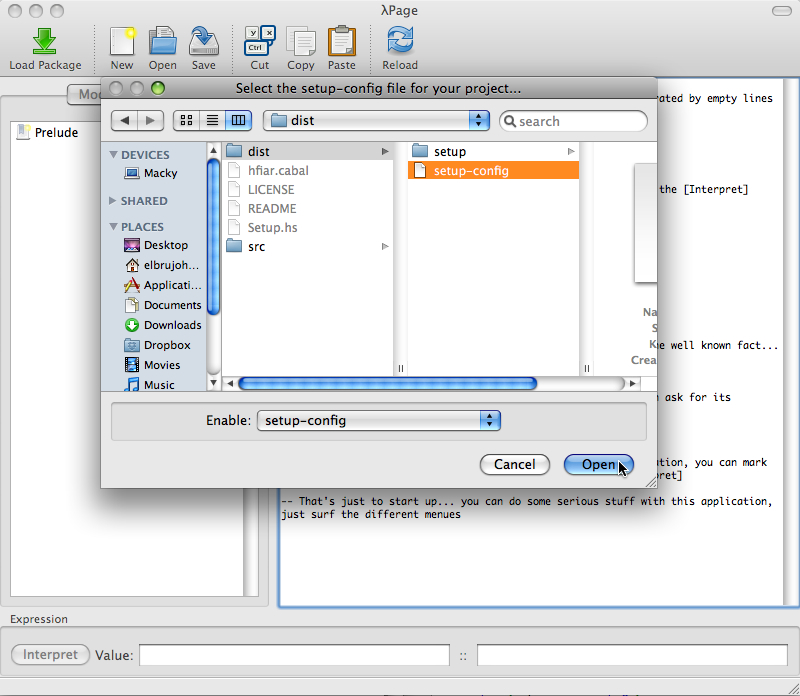
\includegraphics[width=.75\textwidth]{pictures/tut2/02}
		\caption{Tutorial 2 - Cargando un proyecto \cabal}
		\label{tut202}
	\end{center}
\end{figure}
\subparagraph{}F'atima tendr'a entonces a su disposici'on los m'odulos que componen la aplicaci'on y, haciendo click con el bot'on derecho del mouse en ellos, podr'a cargarlos, como se ve en la Figura \ref{tut203}.  \textsl{Cargar} un m'odulo es la acci'on de poner en contexto las funciones y tipos de datos definidos en 'el, de modo que puedan ser utilizados dentro de las p'aginas actuales.  Al \textsl{cargar} un m'odulo, \hpage\ carga recursivamente los m'odulos de los que 'este depende.  Todos los m'odulos previamente cargados, excepto los m'odulos del paquete, se olvidan.  Si existe c'odigo precompilado para el m'odulo, \hpage\ lo utiliza.  En otro caso, intenta compilar su c'odigo desde el archivo fuente.
\begin{figure}[hp]
	\begin{center}
        	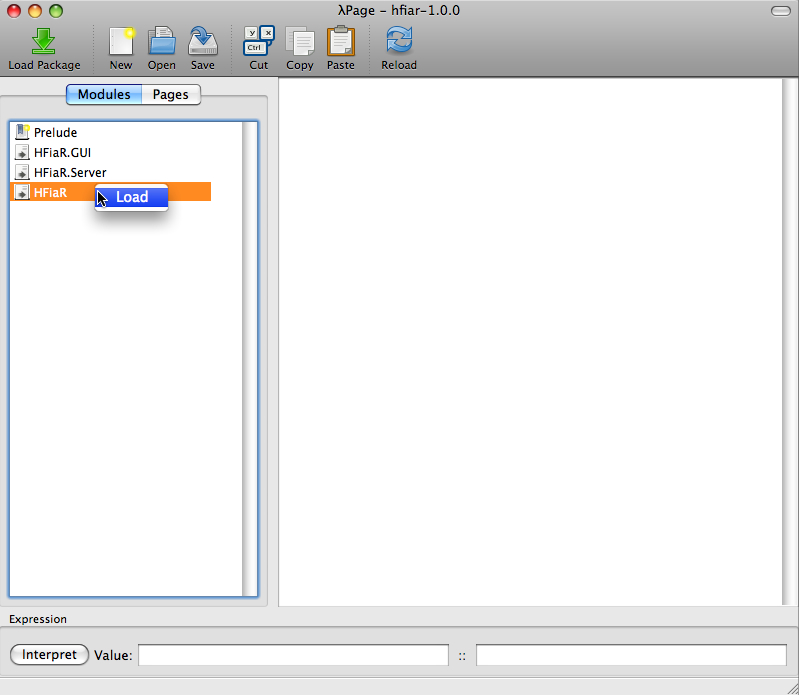
\includegraphics[width=.75\textwidth]{pictures/tut2/03}
		\caption{Tutorial 2 - Proyecto \cabal\ cargado}
		\label{tut203}
	\end{center}
\end{figure}

\newpage
\paragraph{}Recordando que el proyecto inclu'ia una librer'ia compuesta 'unicamente por el m'odulo \texttt{HFiaR}, nuestra amiga F'atima decide cargarlo y navegarlo utilizando el men'u desplegable que nos muestra la Figura \ref{tut204}.
\begin{figure}[hp]
	\begin{center}
        	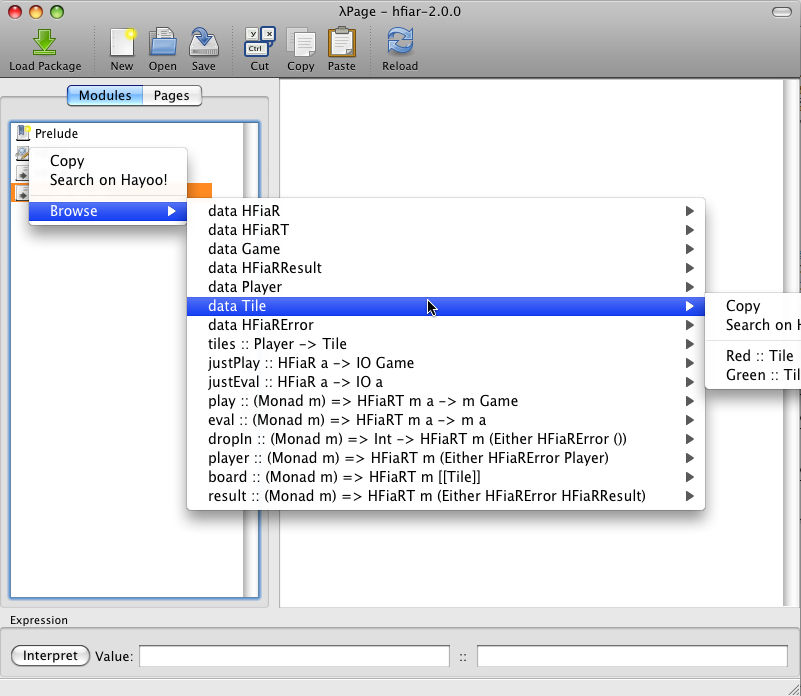
\includegraphics[width=.75\textwidth]{pictures/tut2/04}
		\caption{Tutorial 2 - M'odulo \texttt{HFiaR}}
		\label{tut204}
	\end{center}
\end{figure}
\paragraph{}Gracias a la documentaci'on generada previamente, puede observar que la din'amica del juego est'a modelada con una m'onada~\cite{monads} que describe las acciones llevadas a cabo durante un partido.  El concepto de \textsl{m'onada} (monad) es uno de los m'as dif'iciles de comprender para aquellos que dan sus primeros pasos en \haskell.  A los fines de este tutorial, podemos ver a las m'onadas como tipos de datos que nos permiten definir acciones que generan resultados (por ejemplo, \texttt{dropIn} o \texttt{player} son acciones de la m'onada \texttt{HFiaR}) y concatenarlas utilizando distintos operadores gen'ericos (como \texttt{$>>$}) para generar nuevas acciones m'as complejas (como por ejemplo, \texttt{dropIn 1 $>>$ player}, que es una acci'on de la m'onada \texttt{HFiaR} que representa el hecho de arrojar una ficha en la columna 1 y luego verificar cu'al es el jugador actual).  Estas acciones, luego pueden ser ``ejecutadas''.  En nuestro caso dicha ejecuci'on se realiza, por ejemplo, utilizando las funciones \texttt{play} (cuyo resultado refleja el estado del partido una vez ejecutada las acci'on) o \texttt{eval} (cuyo resultado es el de la acci'on ejecutada).
\subparagraph{}F'atima verifica las funciones de la m'onada \texttt{HFiaR} con las que cuenta:
\begin{description}
	\item[\texttt{dropIn}] representa el hecho de arrojar una ficha en una columna
	\item[\texttt{tryDropIn}] representa el hecho de verificar qu'e pasar'ia en el caso de realizar serie de jugadas, donde cada una de ellas corresponde a arrojar una ficha en una columna.  Es similar a \texttt{dropIn} pero sin que el juego avance
	\item[\texttt{player}] le permite conocer el jugador actual
	\item[\texttt{board}] le permite observar el tablero, que es modelado como una lista de listas de \texttt{Tile}s, o sea fichas)
	\item[\texttt{result}] le permite verificar el resultado del partido, si es que el mismo ha conclu'ido
\end{description}

\subparagraph{}Como el lector, al igual que F'atima, habr'a podido observar en la Figura \ref{tut204}, si bien las acciones que pueden definirse corresponden a la m'onada \texttt{HFiaR}, dado el tipo de \texttt{play} y \texttt{eval}, las mismas pueden ser ejecutadas dentro de cualquier m'onada.  Esto se debe a que la m'onada est'a implementada utilizando la t'ecnica de \textsl{Monad Transformers}~\cite{realworldhaskell}~\cite{mtl}.  Los \textsl{Transformadores de M'onadas} (Monad Transformers) son variantes especiales de las m'onadas que facilitan la combinaci'on de m'onadas.  Sus constructores de tipo tienen como par'ametro un tipo mon'adico y proucen tipos mon'adicos combinados.  En este tutorial, por ejemplo, las funciones \texttt{justPlay} y \texttt{justEval}, est'an definidas internamente utilizando el tipo transformador \texttt{HFiaRT} para ejecutar acciones de la m'onada \texttt{HFiaR} dentro de la m'onada \texttt{IO}.

\subparagraph{}Utilizando estas funciones, F'atima comienza a realizar su tarea de \textsl{micro-testing}.  Su primera prueba consiste en \textit{jugar} un partido en el que nada pasa, s'olo para ver qu'e informaci'on puede obtener de 'el.  Coloca entonces en la p'agina la expresi'on que presentamos a continuaci'on e intenta interpretarla tal como se ve en la Figura \ref{tut205}.  Esta expresi'on, aunque simple, presenta dos elementos muy utilizados por los desarrolladores \haskell: el operador \$, que equivale a encerrar entre par'entesis lo que sigue en la expresi'on, facilitando la lectura de la expresi'on en su totalidad, y la expresi'on \texttt{return ()}, que es la acci'on que representa el hecho de simplemente ``no hacer nada''.  Como toda acci'on debe tener un resultado, la acci'on \texttt{return ()}, el de \texttt{return ()} es \texttt{()}, el 'unico valor posible de tipo \texttt{Unit}.
\lstset{language=haskell, frame=single, tabsize=4}
\begin{center}\begin{lstlisting}
	justPlay $ return ()
\end{lstlisting}\end{center}
\begin{figure}[hp]
	\begin{center}
        	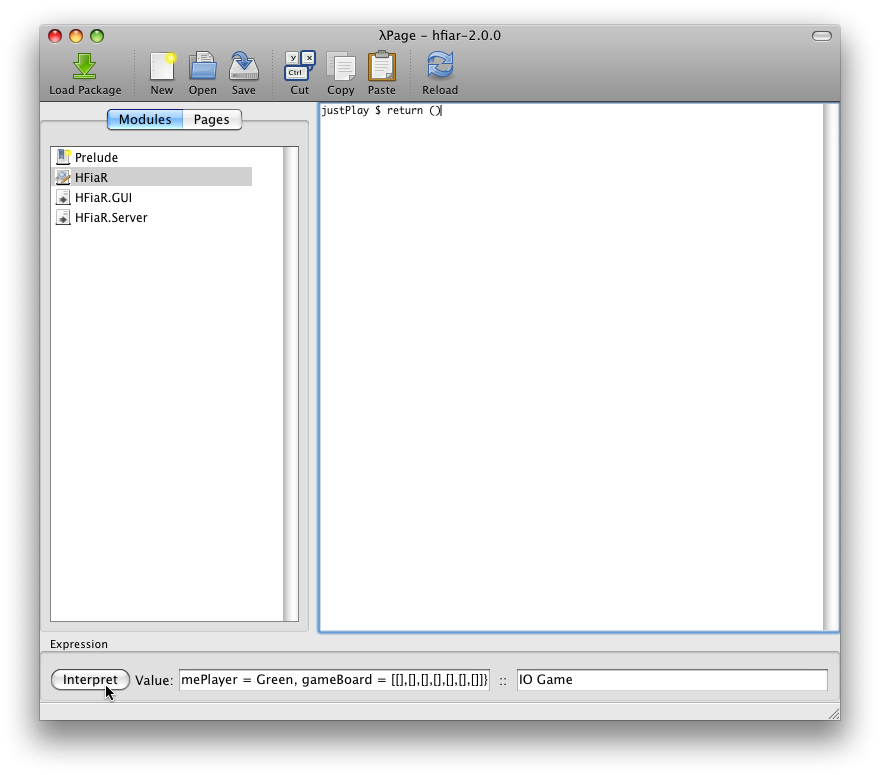
\includegraphics[width=.75\textwidth]{pictures/tut2/05}
		\caption{Tutorial 2 - Juego M'inimo}
		\label{tut205}
	\end{center}
\end{figure}
\subparagraph{}El resultado obtenido es el que sigue y puede interpretarse como \textsl{``el partido se encuentra en curso, es el turno del jugador que juega con fichas verdes y el tablero est'a vac'io''}.  Cabe notar que el tipo del resultado es \texttt{IO Game}, o sea, una acci'on con posibles efectos colaterales de entrada/salida (dentro de la m'onada \texttt{IO}) cuyo resultado es un juego (\texttt{Game}).  Sin embargo, el resultado obtenido representa simplemente a un juego.  Esto se debe a que \hpage, siguiendo el ejemplo de \textsl{GHCi}, trata de manera especial a las acciones de la m'onada \texttt{IO} y, en lugar de intentar mostrarlas (cosa que, por cierto, no podr'ia hacer) las eval'ua y luego intenta mostrar su resultado.
\begin{center}\begin{lstlisting}
OnCourse {gamePlayer = Green,
          gameBoard = [[],[],[],[],[],[],[]]}
\end{lstlisting}\end{center}
\newpage
\paragraph{}Usando \hpage, F'atima realiza varias otras pruebas que consignamos en la tabla que presentamos a continuaci'on.  Con ellas puede entender el funcionamiento general de la m'onada \texttt{HFiaR} y de ese modo determinar c'omo su jugador de inteligencia artificial puede observar el desarrollo del juego (saber si el mismo ha concluido o no, si es su turno y el estado del tablero) y elegir c'omo jugar.  Cabe notar que los resultados de tipo \texttt{Left HFiaRError} se exhiben como texto porque el desarrollador de \textsl{hfiar} ha decidido utilizar la funci'on \texttt{show} para describir los errores en lugar de exhibir su constructor.

\lstset{language=haskell, frame=none, tabsize=4}
	\begin{table}[hp]
		\begin{center}
			\begin{tabular}{@{} cc @{}}
				\toprule
				Expresi'on & Resultado \\ 
				\midrule
\begin{lstlisting}
justPlay $ return ()
\end{lstlisting} &
\begin{lstlisting}
OnCourse {gamePlayer = Green,
          gameBoard = [[],[],[],[],[],[],[]]}
\end{lstlisting} \\[1.5em]

\begin{lstlisting}
justEval player
\end{lstlisting} &
\begin{lstlisting}
Right Green
\end{lstlisting} \\[1.5em]

\begin{lstlisting}
justEval $ dropIn 1 >> board
\end{lstlisting} &
\begin{lstlisting}
[[],[Green],[],[],[],[],[]]
\end{lstlisting} \\[1.5em]

\begin{lstlisting}
justEval $ dropIn 1 >> 
           dropIn 2 >> board
\end{lstlisting} &
\begin{lstlisting}
[[],[Green],[Red],[],[],[],[]]
\end{lstlisting} \\[1.5em]

\begin{lstlisting}
justEval $ dropIn 1 >> dropIn 1 >>
           dropIn 2 >> board
\end{lstlisting} &
\begin{lstlisting}
[[],[Red, Green],[Green],[],[],[],[]]
\end{lstlisting} \\[1.5em]

\begin{lstlisting}
justEval $ dropIn 7
\end{lstlisting} &
\begin{lstlisting}
Left That column doesn't exist
\end{lstlisting} \\[1.5em]

\begin{lstlisting}
justPlay $ dropIn 4 >> dropIn 1 >>
           dropIn 4 >> dropIn 1 >>
           dropIn 4 >> dropIn 1 >>
           dropIn 4
\end{lstlisting} &
\begin{lstlisting}
Ended {gameResult = WonBy Green,
       gameBoard = [[],[Red,Red,Red],
                    [],[],
                    [Green,Green,Green,Green],
                    [],[]]}
\end{lstlisting} \\[1.5em]

\begin{lstlisting}
justEval $ dropIn 4 >> dropIn 1 >>
           dropIn 4 >> dropIn 1 >>
           dropIn 4 >> dropIn 1 >>
           dropIn 4 >> result
\end{lstlisting} &
\begin{lstlisting}
Right (WonBy Green)
\end{lstlisting} \\[1.5em]

\begin{lstlisting}
justEval $ dropIn 4 >> dropIn 1 >>
           dropIn 4 >> dropIn 1 >>
           dropIn 3 >> dropIn 1 >>
           dropIn 4 >> result
\end{lstlisting} &
\begin{lstlisting}
Left Game is still on course
\end{lstlisting} \\[1.5em]

\begin{lstlisting}
justEval $ dropIn 1 >> dropIn 1 >>
           dropIn 1 >> dropIn 1 >>
           dropIn 1 >> dropIn 1 >>
           dropIn 1 >> dropIn 1
\end{lstlisting} &
\begin{lstlisting}
Left That column is full
\end{lstlisting} \\[1.5em]

			\bottomrule
		\end{tabular}
		\caption{Tutorial 2 - Pruebas realizadas en \hpage}
	\end{center}
\end{table}
\lstset{language=haskell, frame=single, tabsize=4}

\newpage
\subsubsection{Creando al \textsl{Jugador Computadora}}
\paragraph{}Con el conocimiento adquirido en el uso de \texttt{HFiaR}, F'atima decide crear la funci'on \texttt{aiDropIn}, que se ejecutar'a dentro de la m'onada \texttt{HFiaR}.  A continuaci'on observamos el tipo de dicha funci'on.  Se puede ver que el tipo de la funci'on es similar al de \texttt{dropIn}, salvo por el hecho de no recibir el n'umero de columna en la que el jugador desea volcar su ficha.  Eso se debe, justamente, a que ser'a la propia funci'on qui'en lo determine.
\begin{center}\begin{lstlisting}
-- | Drop a tile in a column choosen by the Artificial Inteligence
aiDropIn :: Monad m => HFiaRT m (Either HFiaRError ())
\end{lstlisting}\end{center}
\subparagraph{}Para crear \texttt{aiDropIn}, F'atima no cierra \hpage.  Por el contrario, define la funci'on all'i mismo, como podemos ver en la Figura \ref{tut207}, componi'endola con otra funci'on a la que denomina \texttt{bestColumn}.  Esta funci'on se ejecutar'a s'olo en el caso de que el partido no haya concluido.  La idea es que en ella estar'a el algoritmo principal de selecci'on de columna a jugar (o sea, el verdadero motor de \textsl{inteligencia artificial}), el cual se ir'a perfeccionando a lo largo del tutorial.  La primera versi'on de \texttt{bestColumn}, con m'as de artificial que de inteligencia, simplemente elegir'a la primer columna que no est'e llena y \texttt{aiDropIn} arrojar'a la ficha ah'i.  Recordamos que, para que \hpage\ reconozca las distintas expresiones, F'atima debe separarlas con renglones en blanco.
\begin{figure}[hp]
	\begin{center}
        	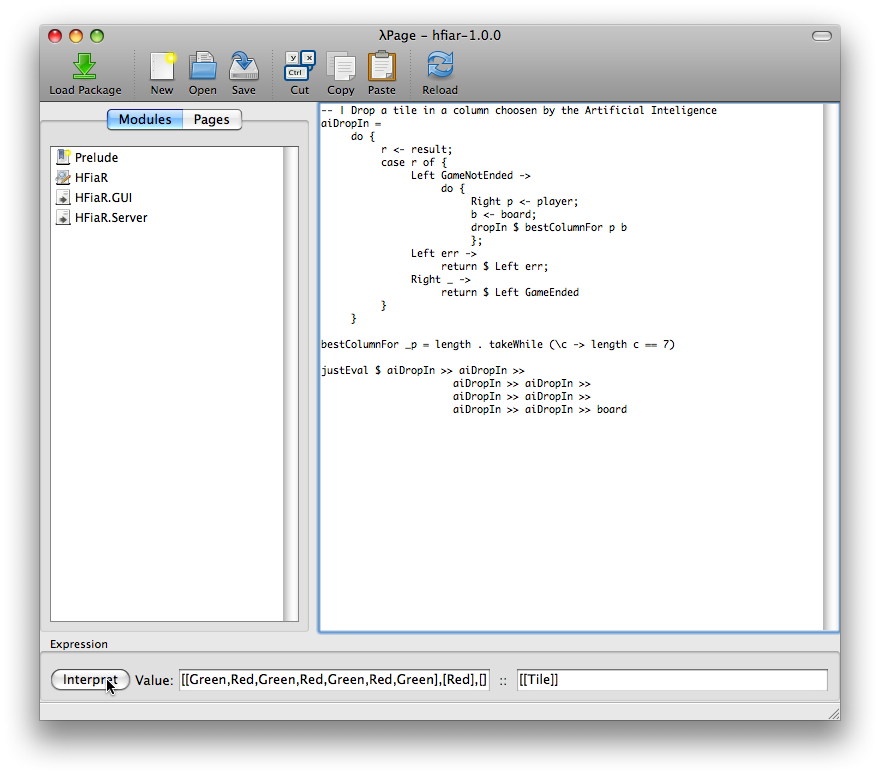
\includegraphics[width=.75\textwidth]{pictures/tut2/06}
		\caption{Tutorial 2 - \texttt{aiDropIn} versi'on 1}
		\label{tut207}
	\end{center}
\end{figure}

\newpage
\subparagraph{}Una vez definidas ambas funciones, F'atima decide testearlas y, para ello, no necesita m'as que \textsl{evaluar} un juego en el que conozca el resultado.  En particular, F'atima elije hacer jugar a la computadora contra s'i misma 8 movimientos y verifica que las fichas han quedado intercaladas en la primer columna y luego el siguiente jugador ha colocado una en la segunda.
\paragraph{}El siguiente paso es agregar un poco de inteligencia a \texttt{bestColumn} de modo que realmente sea competitivo.  Para ello, F'atima prev'e que necesitar'a varias funciones auxiliares y una buena cantidad de c'odigo, por lo que decide convertir su p'agina actual en un m'odulo al que denomina \texttt{HFiaR.AI} y graba en el lugar correspondiente entre los fuentes del proyecto, utilizando la opci'on \textsl{Page $\rightarrow$ Save As\ldots} o el bot'on \textsl{Save}.  A partir de ese momento, F'atima puede utilizar su editor \haskell\ favorito para agregar la cabecera del m'odulo, la importaci'on del m'odulo que ten'ia cargado (\texttt{HFiaR}) y ``bautizar'' la expresi'on utilizada para testear como \texttt{testGame}.  Luego lo carga utilizando la opci'on \textsl{Haskell $\rightarrow$ Load Modules\ldots} y entonces, en una p'agina nueva (creada utilizando la opci'on \textsl{Page $\rightarrow$ New}) escribe e interpreta la expresi'on \texttt{testGame}, de modo de realizar la misma prueba de la Figura \ref{tut207}.  Es interesante notar que, pese a que el m'odulo creado s'olo exporta la funci'on \texttt{aiDropIn}, F'atima pudo interpretar sin problemas la funci'on \texttt{testGame}, pues hab'ia cargado el m'odulo y eso le da acceso a todas las funciones del mismo, tanto p'ublicas como privadas.  A partir de este momento, F'atima utiliza su editor favorito para trabajar en el m'odulo que ha creado y, ante cada modificaci'on del mismo, lo recarga utilizando la opci'on \textsl{Haskell $\rightarrow$ Reload} o el bot'on \textsl{Reload}.
\subparagraph{}Para la segunda (y a los fines de este tutorial, definitva) versi'on de \texttt{bestColumn}, experta jugadora de 4 en l'inea como es, pone un poco de criterio y decide que la funci'on tenga en cuenta las condiciones que enumeramos a continuaci'on:
\begin{itemize}
	\item Si poniendo la ficha en alguna columna el jugador gana el partido, se debe elegir esa columna.
	\item Si poniendo la ficha en alguna columna se impide que el jugador rival gane el partido (pues acumula 3 alineadas convenientemente) se debe elegir esa columna.
	\item En otro caso, de ser posible, debe elegirse la columna 3 (o sea, la columna central) pues para formar l'ineas de 4 fichas horizontales o diagonales se requiere una ficha en dicha columna
\end{itemize}

\newpage
\subparagraph{}Podemos observar entonces la nueva versi'on de \texttt{bestColumn} y sus funciones adicionales:
\begin{center}\begin{lstlisting}
module HFiaR.AI (aiDropIn) where

import HFiaR
import Data.Maybe

bestColumn :: Monad m => HFiaRT m Int
bestColumn =
    do
        j1 <- columnWhereWins
        j2 <- columnWhereLoses
        j3 <- column3IfAvailable
        j4 <- firstAvailableColumn
        return . head $ catMaybes [j1, j2, j3, j4]

columnWhereWins, columnWhereLoses,
    column3IfAvailable, firstAvailableColumn :: Monad m => HFiaRT m (Maybe Int)

columnWhereWins = mapM (tryDropIn . (:[])) [0..6] >>= return . firstEnded

columnWhereLoses = mapM moves [0..6] >>= return . firstEnded
    where moves :: Monad m => Int -> HFiaRT m (Either HFiaRError Game)
          moves col = do
            b <- board
            let avail c = c == col || length (b!!c) == 7
            other <- return . length $ takeWhile avail [0..6]
            tryDropIn [other, col]

column3IfAvailable = board >>= \b -> return $ case length (b !! 3) of
                                                    7 -> Nothing
                                                    _ -> Just 3

firstAvailableColumn = board >>=
						return . Just . length . takeWhile (\c -> length c == 7)

firstEnded :: [Either HFiaRError Game] -> Maybe Int
firstEnded games = case (length $ takeWhile onCourse games) of
                        7 -> Nothing
                        g -> Just g
    where onCourse (Left _)           = False
          onCourse (Right OnCourse{}) = True
          onCourse (Right Ended{})    = False
\end{lstlisting}\end{center}
\subparagraph{} Muchas porciones del c'odigo que acabamos de exponer pueden resultar desconocidas o quiz'as dif'iciles de comprender incluso para un programador \haskell\ ya habituado a este tipo de c'odigo.  Tomemos, por ejemplo, la funci'on \texttt{catMaybes}, utilizada en la nueva versi'on de \texttt{bestColumn}.  A los fines de continuar con nuestra historia y demostrar el uso de \hpage, supongamos que, si bien F'atima sab'ia de la existencia de esta funci'on, no sab'ia en qu'e m'odulo se encontraba declarada ni recordaba exactamente su tipo.  En tal caso, lo que F'atima puede hacer es escribir el nombre de la funci'on en la p'agina de \hpage, seleccionarlo y utilizar la opci'on \textsl{Search on Hayoo!} del men'u contextual que se despliega al presionar el bot'on derecho del mouse sobre el texto seleccionado.  En ese momento, \hpage\ le presentar'a la p'agina web que se ve en la Figura \ref{tut209}. All'i se puede observar que la funci'on \texttt{catMaybes} se encuentra definida en el m'odulo \texttt{Data.Maybe} y que su tipo es \texttt{[Maybe a] -> [a]}.  M'as a'un, \textsl{Hayoo!} nos muestra la documentaci'on que acompa'na a la funci'on, seg'un la cual \textit{la funci'on \texttt{catMaybes} toma una lista de \texttt{Maybe}s y devuelve una lista de todos los valores construidos con \texttt{Just}}.  Para probarla, F'atima puede importar el m'odulo \textsl{Data.Maybe} utilizando la opci'on \textsl{Haskell $\rightarrow$ Import modules\ldots} y realizar alguna prueba similar a la de la Figura \ref{tut210}.  El lector podr'ia preguntarse en este momento por qu'e F'atima debi'o importar el m'odulo en lugar de cargarlo como ha hecho con los dem'as m'odulos.  Esto se debe a que el m'odulo \textsl{Data.Maybe} se encuentra en un paquete que no es aquel con el que estamos trabajando, por lo tanto \hpage\ no tiene acceso a su c'odigo fuente.  \textsl{Importar} un m'odulo es similar a cargarlo: es la acci'on de poner en contexto las funciones y tipos de datos definidos y \textbf{exportados} por 'el, de modo que puedan ser utilizados dentro de las p'aginas actuales.  Al importar un m'odulo, el usuario no tiene acceso a las funciones y tipos de datos \textsl{privados} del mismo.
\begin{figure}[hp]
	\begin{center}
        	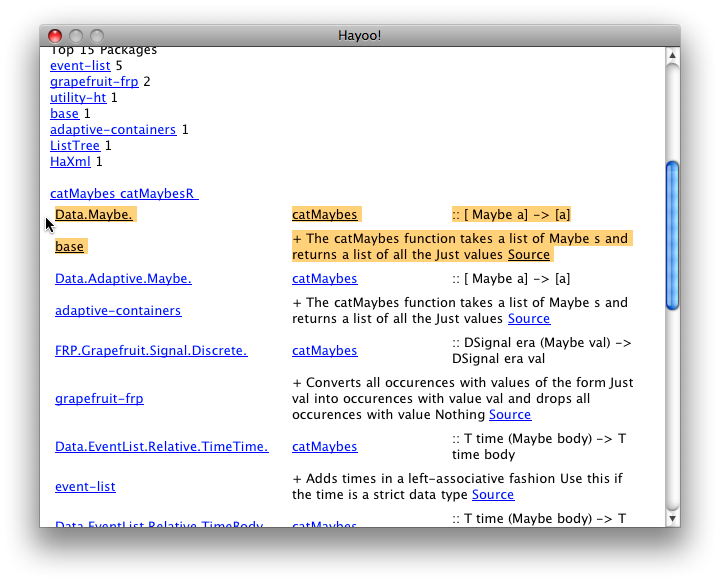
\includegraphics[width=.75\textwidth]{pictures/tut2/09}
		\caption{Tutorial 2 - Utilizando \textsl{Hayoo!}}
		\label{tut209}
	\end{center}
\end{figure}
\begin{figure}[hp]
	\begin{center}
        	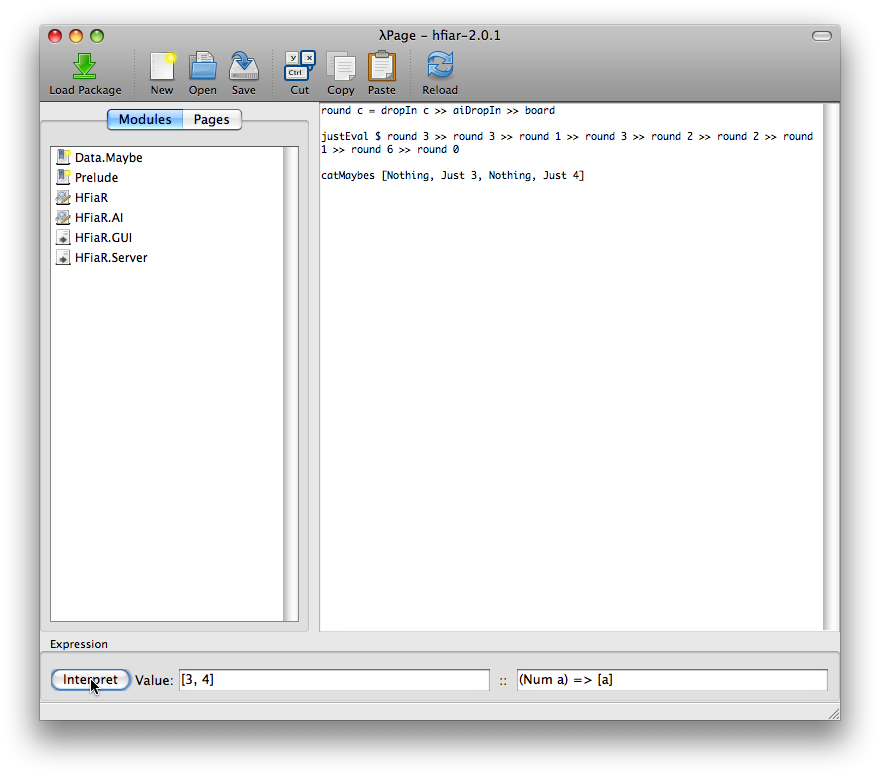
\includegraphics[width=.75\textwidth]{pictures/tut2/10}
		\caption{Tutorial 2 - Testeando \texttt{catMaybes}}
		\label{tut210}
	\end{center}
\end{figure}

\newpage
\paragraph{} La funci'on \texttt{testGame} ya no es suficiente para testear el funcionamiento de \texttt{aiDropin} pero, como el c'odigo est'a en un m'odulo que ha sido cargado dentro de \hpage, lo que F'atima puede hacer es ir construyendo paso a paso una expresi'on que represente un partido entre ella y \textsl{el Jugador Computadora}.  Para ello, define la funci'on auxiliar \texttt{round} y, tal como lo vemos en la Figura \ref{tut211}, la utiliza una y otra vez para modificar el partido que pretende ``jugar''.  De ese modo puede probar el comportamiento de su m'odulo de inteligencia artificial ante las distintas circunstancias de un partido tan extenso como ella desee.  Cabe destacar una vez m'as aqu'i que, cada vez que F'atima desee realizar cambios en su m'odulo, puede hacerlo con su editor favorito, luego presionar el bot'on \textsl{Reload} al volver a \hpage\ e interpretar nuevamente sus expresiones, que no han sido perdidas pues est'an todav'ia en la(s) p'agina(s) con la(s) que est'a trabajando.
\begin{figure}[hp]
	\begin{center}
        	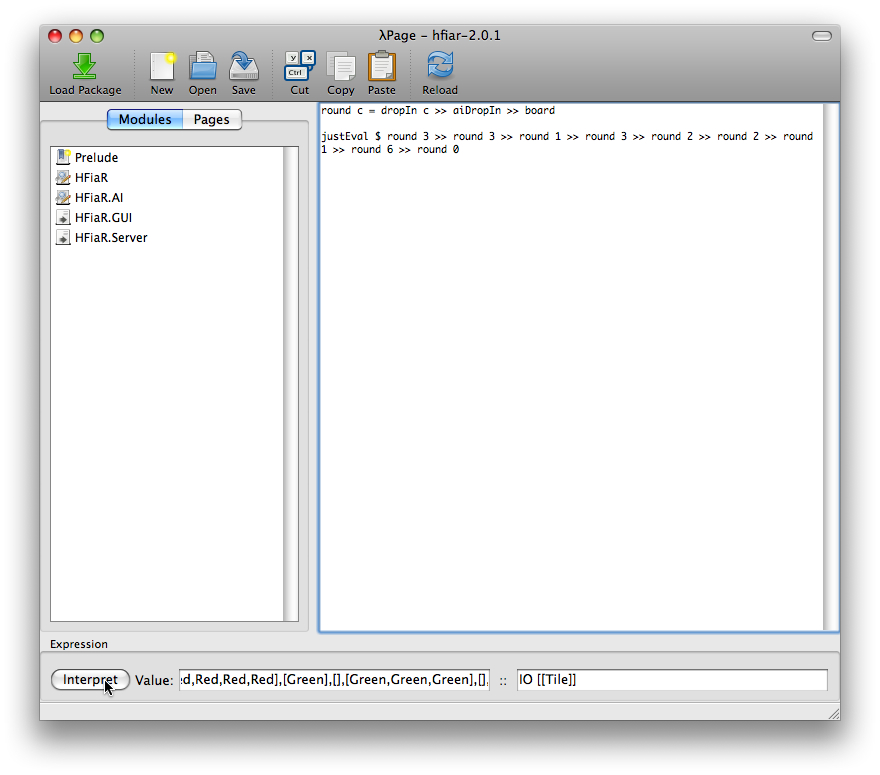
\includegraphics[width=.75\textwidth]{pictures/tut2/08}
		\caption{Tutorial 2 - \textsl{Jugando} contra \texttt{HFiaR.AI}}
		\label{tut211}
	\end{center}
\end{figure}
\paragraph{}Resta pues modificar la interfaz gr'afica para que permita al usuario jugar contra la computadora, utilizando la funci'on \texttt{aiDropIn} en los turnos correspondientes a la m'aquina.  Para ello, F'atima abre el m'odulo \texttt{HFiaR.GUI} y realiza los cambios pertinentes.   Se trata b'asicamente de modificaciones de la interfaz gr'afica del programa, para las cuales \hpage\ no es de m'as ayuda que en los ejemplos que hemos visto a lo largo de este tutorial.  Por ese motivo no los detallamos en este informe.  Para quien desee observarlos puede encontrarlos en \htmladdnormallink{la p'agina web del proyecto hfiar en github}{bihttp://github.com/elbrujohalcon/hfiar/commit/d69ab637bf32866e7e4550b6ea51cdd5fba33a90\#diff-2}~\cite{hfiar}
\paragraph{}El 'ultimo paso que F'atima debe realizar es incluir su nuevo m'odulo en la lista de m'odulos de la librer'ia \textsl{HFiaR} dentro del archivo \textbf{hfiar.cabal}.  Una vez hechas estas modificaciones, puede ejecutar los siguientes comandos y disfrutar de un partido de su juego favorito contra la computadora:
\lstset{language=sh, frame=single, tabsize=4}
\begin{center}\begin{lstlisting}
$ cabal configure --user
$ cabal build
$ cabal install
$ ~/.cabal/bin/hfiar &
\end{lstlisting}\end{center}

\newpage
\subsubsection{Conclusiones}
\paragraph{}A lo largo de este tutorial hemos podido ver c'omo utilizar \hpage\ para \textsl{comprender} c'odigo \haskell\ a trav'es de \textsl{micro-testing}.  Hemos visto tambi'en como, utilizando esa misma t'ecnica, podemos construir paso a paso m'odulos \haskell\ medianamente complejos.  Pudimos ver c'omo \hpage\ nos permite editar los m'odulos y recargarlos para volver a testearlos sin perder las expresiones que ya hab'iamos definido.
\paragraph{}Hemos podido ver c'omo \hpage\ se encuentra integrado con \cabal\ para permitir cargar proyectos previamente configurados y evitar al desarrollador lidiar con el manejo de extensiones, carpetas y m'odulos manualmente.  Esto es una importante ventaja que ofrece \hpage\, dado que la mayor'ia de los proyectos desarrollados en \haskell\ se encuentran organizados en paquetes \cabal.  Pudimos observar tambi'en c'omo \hpage\ se integra con \textsl{Hayoo!}, permitiendo al desarrollador consultar sus dudas sobre la API de \haskell directamente dentro de la aplicaci'on.
\paragraph{}Hemos observado c'omo utilizar \hpage\ para cargar o importar m'odulos y hemos notado las diferencias entre estas dos acciones.  Tambi'en hemos observado la forma gr'afica con la que \hpage\ describe y permite navegar los m'odulos cargados o importados, sus funciones y sus estructuras de datos para luego utilizarlas en nuestro c'odigo.
\paragraph{}Por otra parte, hemos podido trabajar con expresiones de entrada/salida que podr'ian generar efectos colaterales (en otras palabras, expresiones de tipo \texttt{IO a}) de manera transparente, tal como lo har'iamos con \textsl{GHCi}.

\newpage
\subsection{Otras Caracter'isticas de \hpage}
\begin{epigraphs}
	%%TODO: Epigrafear
	\qitem{TODO: EP'IGRAFE}{autor}
\end{epigraphs}
\paragraph{}Los dos tutoriales que hemos presentado en este cap'itulo muestran muchas de las principales caracter'isticas de \hpage.  Sin embargo, algunas otras caracter'isticas han quedado sin ser expuestas.  Es nuestra intenci'on utilizar esta secci'on para detallarlas, de modo que el usuario interesado pueda experimentar con ellas.
\subsubsection{Listas} %%TODO: TEXTO
\subsubsection{Resultados Parciales}\label{secTutWIC} %%TODO: WIC
\lstset{language=haskell, frame=single, tabsize=4}
\begin{center}\begin{lstlisting}
data WithInfiniteChar = WIC

instance Show WithInfiniteChar where
    show WIC = ['c', head . show $ length [1..]]
\end{lstlisting}\end{center}
\subparagraph{}Como puede observarse, al intentar mostrar la expresi'on \texttt{WIC}, \hpage\ se encontrar'a con una cadena cuyo segundo caracter no puede computar pues requiere un c'alculo infinito, en la figura representamos este caracter con la letra $\Omega$.  All'i es donde entra en acci'on el \textbf{Runaway Killer} para informar esta situaci'on al usuario.
\subsubsection{Kind} %%TODO: TEXTO
\subsubsection{Importaci'on de M'odulos por Nombre} %%TODO: TEXTO
\subsubsection{Configuraci'on del Compilador} %%TODO: TEXTO

\newpage
\section{Desarrollo - ?`C'omo se hizo \hpage?}
\subsection{Arquitectura General}
\begin{epigraphs}
	\qitem{If you think good architecture is expensive, try bad architecture}{Brian Foote and Joseph Yoder}
\end{epigraphs}
\paragraph{}Las principales decisiones de arquitectura que se tomaron durante el desarrollo de \hpage\ tuvieron como principales motivaciones los siguientes requerimientos:
\begin{description}
\item[Conexi'on con GHC] \hpage\ deb'ia conectarse con el motor de GHC a trav'es de su API de modo de poder detectar e interpretar expresiones.  Para ello se utiliz'o \htmladdnormallink{hint}{http://projects.haskell.org/hint}~\cite{hint}.  \textsl{hint} es una librer'ia hecha en \haskell\ que provee una abstracci'on de alto nivel sobre la API de GHC.  Esta librer'ia nos permite acceder de modo sencillo a las funciones provistas por la API y as'i poder evaluar expresiones, determinar su tipo y, en caso de expresiones de tipo, su g'enero, cargar e importar m'odulos, utilizar extensiones del lenguaje y opciones del compilador.  \textsl{hint} provee funciones que permiten este manejo y pueden ser ejecutadas dentro de la m'onada \texttt{Interpreter}.
\item[Paralelismo] \hpage\ deb'ia permitir al usuario editar sus p'aginas mientras esperaba el resultado de la evaluaci'on de una expresi'on, detectar evaluaciones que podr'ian ser infinitas y presentar la interpretaci'on de una expresi'on de manera incremental.  Todas estas tareas requieren la ejecuci'on de acciones en paralelo.  Para simplificar estas tareas, se cre'o \textsl{eprocess} y se implement'o un modelo de procesos utiliz'andolo.  En la Secci'on \ref{secImplement} podremos observar en detalle c'omo ha sido desarrollada esta librer'ia.
\item[Errores Controlados] \hpage\ no deb'ia fallar si la evaluaci'on de una expresi'on fallaba.  M'as a'un, tambi'en deb'ia detectar posibles evaluaciones infinitas e informar estas situaciones al usuario.  Aqu'i nuevamente entran en juego tanto \textsl{hint} como \textsl{eprocess}.
\item[Compatibilidad con GHCi] \hpage\ deb'ia ser capaz de reemplazar a \textsl{GHCi} y, por lo tanto, brindar toda las funcionalidades que esta aplicaci'on brinda.  En particular, deb'ia:
	\begin{itemize}
		\item ser multiplataforma
		\item detectar expresiones sint'acticamente inv'alidas
		\item identificar el tipo de cualquier expresi'on sint'acticamente v'alida
		\item identificar la clase de cualquier tipo sint'acticamente v'alido
		\item interpretar expresiones de cualquier tipo que sea instancia de la clase \textbf{Show}
		\item ejecutar e imprimir el resultado de expresiones de tipo \textbf{Show a $\Rightarrow$ IO a}
	\end{itemize}
\end{description}
\begin{figure}[hp]
	\begin{center}
        	\fbox{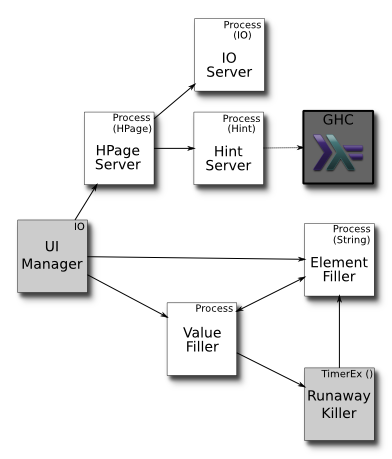
\includegraphics{pictures/architecture}}
		\caption{Arquitectura de \hpage}
		\label{arq1}
	\end{center}
\end{figure}
\subparagraph{}Teniendo en cuenta estos requerimientos, la arquitectura resultante puede ser descripta con el diagrama de la Figura \ref{arq1}.  Esta figura presenta el estado del sistema en un instante dado.  Cada bloque representan un proceso o ``thread'' en ejecuci'on. %%TODO: Explicar que no son threads del Sistema Operativo (copiar de RealWorldHaskell o algo as�)
\subparagraph{}Cada uno de estos procesos se ejecuta dentro del entorno de una m'onada, la cual se encuentra identificada en la esquina superior derecha del bloque.  En el diagrama podemos identificar los siguientes componentes:
\begin{description}
	\item[UI Manager] Este es el thread que inicia el programa, genera y administra la interfaz del usuario utilizando las herramientas provistas por \textsl{wxHaskell}.  En este thread se mantiene el estado visual de la aplicaci'on: el estado de los controles, la 'ultima b'usqueda realizada, etc.
	\item[HPage Server] Este proceso, iniciado por el \textbf{UI Manager}, es el que comunica a la interfaz del usuario con la m'aquina virtual de GHC, a trav'es del \textbf{Hint Server}.  En el caso de expresiones de tipo \textbf{IO a}, este mismo proceso se comunica con el \textbf{IO Server} para ejecutarlas y obtener su resultado o capturar sus errores.  En este proceso se mantiene el estado general de la aplicaci'on: sus p'aginas, expresiones, paquetes y m'odulos cargados, etc.  Este proceso permite la ejecuci'on de acciones definidas en la m'onada \texttt{HPage} de manera sincr'onica o asincr'onica.  En el caso de acciones ejecutadas asincr'onicamente, permite que las mismas sean canceladas.  En tales casos, dado que la API de \textsl{GHC} no provee un mecanismo para cancelar la acci'on en curso, \textbf{HPage Server} reinicia el \textbf{Hint Server} y se encarga de ``ponerlo al d'ia'' aplicando las acciones necesarias para que se encuentre en el estado anterior a la ejecuci'on de la 'ultima acci'on.
	\item[IO Server]Este proceso, iniciado por el  \textbf{HPage Server}, es el encargado de ejecutar acciones de tipo \textbf{IO a} en un entorno controlado y obtener su resultado.
	\item[Hint Server] Este proceso, iniciado por el \textbf{HPage Server}, mantiene una conexi'on con la m'aquina virtual de GHC (a la cual se muestra en la figura conectado a trav'es de una l'inea de puntos)
	\item[Char Filler] Este proceso, iniciado por el \textbf{UI Manager} cumple una muy sencilla funci'on: utilizando los procedimientos de env'io y recepci'on de mensajes provistos por \textsl{eprocess}, espera recibir un caracter (o sea, una expresi'on de tipo Char), para luego evaluarlo y enviar como respuesta su valor en forma normal.
	\item[Value Filler] Este proceso, iniciado por el \textbf{UI Manager} es el encargado de procesar el resultado obtenido del \textbf{HPage Server}.  Cabe recordar aqu'i que \haskell\ trabaja con evaluaci'on ``lazy'', por lo cual el resultado obtenido no ha sido a'un completamente procesado.  El \textbf{Value Filler} espera recibir un resultado y, al recibirlo, se encarga de evaluarlo y mostrarlo por pantalla, para ello env'ia y recibe mensajes del \textbf{Char Filler} a fin de procesar cada caracter a mostrar.
	\item[Runaway Killer] Este thread, creado utilizando la clase \textsl{TimerEx} provista por \textsl{wxHaskell}, es iniciado por cada \textbf{Value Filler} al momento de enviar un nuevo caracter al \textbf{Char Filler}.  El objetivo del \textbf{Runaway Killer} es el de detectar procesamiento ``posiblemente'' infinito.  B'asicamente, pasado un segundo de procesamiento, reinicia el \textbf{Char Filler} e informa al \textbf{Value Filler} que lo inici'o que el caracter que se esperaba procesar ha demorado demasiado y podr'ia desencadenar una evaluaci'on infinita.
\end{description}
\paragraph{}Para un mayor detalle, la Figura \ref{seq1} nos muestra un diagrama de secuencia correspondiente a un proceso de evaluaci'on.  Para poder brindar un ejemplo completo, observaremos la evaluaci'on de una lista en la que algunos de sus valores generan error.
%%TODO: Nuevo cuadro de secuencia
\begin{figure}[hp]
	\begin{center}
        	\fbox{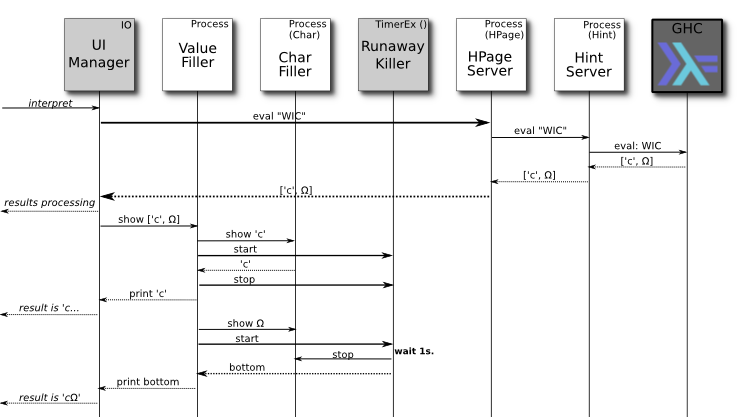
\includegraphics[width=\textwidth]{pictures/sequence}}
		\caption{Secuencia de Evaluaci'on de [1, undefined, 3, undefined]}
		\label{seq1}
	\end{center}
\end{figure}

\newpage
\subsection{Dise'no}
\begin{epigraphs}
	\qitem{Design and programming are human activities; forget that and all is lost}{Bjarne Stroustrup}
\end{epigraphs}
\paragraph{}Presentaremos a continuaci'on las principales decisiones de dise'no que se han tomado durante la creaci'on de \hpage.  Todas ellas tienen como fundamento los requerimientos principales exhibidos en la secci'on anterior y tambi'en algunos requerimientos adicionales, como la integraci'on con \cabal\ y \textsl{Hayoo!}.
\subsubsection{Concurrencia}
\paragraph{}Como hemos visto en la secci'on anterior, al momento de dise'nar \hpage\ tuvimos que considerar la necesidad de paralelizar tareas, para permitir al usuario, por ejemplo, trabajar en un documento mientras el motor de \hpage\ eval'ua una expresi'on.  Tambi'en debemos considerar que estas tareas a realizar en paralelo no son totalmente independientes sino que requieren una sincronizaci'on.  Tomando la idea del modo en que est'a dise'nado el lenguaje de programaci'on \textsl{Erlang}, decidimos implementar el paralelismo utilizando lo que denominamos \textsl{procesos}.  Conceptualmente, los \textsl{procesos} son hilos de ejecuci'on que se realizan en paralelo y pueden recibir o enviar mensajes.   Esta caracter'istica de mensajer'ia entre procesos es la que permite la sincron'ia cuando es necesaria.  Por otra parte, a diferencia de \textsl{Erlang}, al utilizar \haskell, los mensajes enviados de un proceso a otro pueden ser mucho m'as complejos.  Gracias al hecho de que en \haskell\ las acciones son elementos de primer orden, un proceso puede enviar a otro directamente las acciones que desea que 'este ejecute, tal como deben ser ejecutadas.  Esta es una caracter'istica esencial para reducir la complejidad de la implementaci'on de todos nuestros procesos, en particular de aquellos que act'uan como servidores (\textbf{IO Server}, \textbf{HPage Server} y \textbf{Hint Server}), como veremos luego en la Secci'on \ref{secImplement}.
\subsubsection{Bottoms}
\paragraph{}El lenguaje \haskell\ tiene una caracter'istica 'unica: \textsl{la evaluaci'on perezosa} o \textsl{lazy evaluation}.  Gracias a esta caracter'istica, las expresiones \haskell\ no son completamente evaluadas (reducidas a forma normal) hasta el momento en que realmente se necesita conocer su valor.  Dado que \hpage\ presenta al usuario un interprete de expresiones, es necesario que est'e preparado para no s'olo soportar sino tambi'en aprovechar esta caracter'istica.  En particular, dentro de \hpage\ las expresiones son reducidas a forma normal al momento de intentar mostrar el resultado de su evaluaci'on al usuario.  En ese momento, \hpage\ distingue cuatro tipos de valores:
\begin{description}
	\item[Listas] Expresiones cuyo valor es de tipo \texttt{[a]}, donde \texttt{a} es un tipo que es instancia de la clase \texttt{Show}.  En este caso, \hpage\ intenta reducir cada elemento e ir present'andolo al usuario dentro de una lista.  Cada elemento entonces, es tratado como se ver'a a continuaci'on.
	\item[Entrada/Salida] Expresiones cuyo valor es de tipo \texttt{IO a}, donde \texttt{a} es un tipo que es instancia de la clase \texttt{Show}.  En este caso, \hpage\ intentar'a ejecutar la acci'on, obtener su resultado y presentarlo al usuario como se ver'a a continuaci'on.
	\item[Expresiones ``visibles''] Expresiones cuyo tipo es instancia de la clase \texttt{Show}.  \hpage\ intenta evaluar la expresi'on a mostrar y pueden suceder varias cosas:
		\begin{itemize}
			\item Por supuesto, puede suceder que al evaluar la expresi'on se obtenga una cadena de caracteres, en cuyo caso \hpage\ simplemente presentar'a el resultado al usuario
			\item Puede suceder que, intentando evaluar la expresi'on se obtenga una cadena de caracteres de longitud infinita.  La pol'itica de \hpage\ en este caso es permitir al usuario decidir cu'ando desea abortar la evaluaci'on y mostrar la porci'on del resultado obtenida hasta ese momento
			\item Puede suceder tambi'en que, intentando evaluar un caracter, se genere un c'alculo ``infinito'' o una excepci'on.  En este caso tambi'en, \hpage\ permite al usuario cancelar la evaluaci'on cuando lo considere apropiado.
			\item Otra posibilidad es que, luego de presentar un caracter, al intentar obtener el resto de la cadena, \hpage\ encuentre un c'alculo ``infinito''.  En estos casos, nuevamente \hpage\ permite al usuario cancelar la evaluaci'on cuando lo considere apropiado.
			\item Por 'ultimo, es posible que, luego de presentar un caracter, al intentar obtener el resto de la cadena, \hpage\ encuentre una excepci'on.  En estos casos, \hpage\ informa la situaci'on al usuario y aborta la evaluaci'on de la expresi'on.
		\end{itemize}
	\item[Expresiones no ``visibles''] Expresiones cuyo tipo no es instancia de la clase \texttt{Show}.  \hpage\, ante estas expresiones, se limita a mostrar su tipo.
\end{description}
\subparagraph{}La distinci'on que hace \hpage\ ante los distintos tipos de expresiones  a procesar y el comportamiento escogido al momento de mostrar el resultado de su evaluaci'on tienen como objetivo brindar al usuario la mayor cantidad de informaci'on posbile sobre la expresi'on que desea interpretar.  Sin ellos, el comportamiento natural de un programa como \hpage\ ante una expresi'on \texttt{e}, ser'ia el de asignar el resultado de \texttt{show e} al cuadro de texto que presenta el resultado al usuario.
\subparagraph{}En el caso de las acciones de entrada/salida, \hpage\ al igual que \textsl{GHCi}, considera que el usuario no est'a simplemente interesado en conocer el tipo de las acciones, sino en ejecutarlas para producir (de ser preciso) ciertos efectos secundarios y obtener un resultado.  Es razonable pensar que quien construye una acci'on de este tipo (que no es instancia de la clase \texttt{Show}) pero que produce (al ser evaluada) un resultado de un tipo que s'i lo es, est'a interesado en ejecutar la acci'on y observar el resultado.
\subparagraph{}Observemos con un ejemplo, qu'e suceder'ia.  Para nuestro ejemplo, vamos a crear un tipo de datos similar al que creamos en la Secci'on \ref{secTutWIC}, pero esta vez, le agregaremos un par'ametro:
\begin{center}\begin{lstlisting}
data WithInfiniteChar2 = WIC2 Int

instance Show WithInfiniteChar2 where
    show (WIC2 x) | x < 0 = ['c', head $ show x]
			  | x == 0 = undefined
			  | otherwise = ['c', head . show $ length [1..]]

test = map WIC2 [-5,-4..]
\end{lstlisting}\end{center}
\subparagraph{}Si el usuario quisiese interpretar la expresi'on \texttt{[-5, -4..]} y \hpage\ intentase asignar \texttt{show [-5, -4..]} al cuadro de texto, el int'erprete reducir a forma normal una lista infinita, c'alculo que nunca terminar'ia y por tanto, el usuario no ver'ia ning'un resultado en la pantalla.
\subparagraph{}Si, en su lugar, el usuario quisiese interpretar la expresi'on \texttt{test}, el int'erprete generar'ia una excepci'on \texttt{Prelude.undefined} al intentar mostrar el sexto elemento de la lista (el correspondiente a \texttt{0} en la lista original) y esa excepci'on ser'ia todo lo que el usuario podr'ia saber sobre la evaluaci'on de su expresi'on.
\subparagraph{}Entonces, en vez de asignarlo directamente, \hpage\ podr'ia evaluar la expresi'on caracter a caracter e ir presentando cada uno de ellos al usuario a medida que los va obteniendo.  En ese caso, los caracteres correspondientes a los primeros 5 elementos de la lista (\texttt{[c-,c-,c-,c-,c-,}) podr'ian ser mostrados al usuario, pero al llegar al sexto, nuevamente el int'erprete generar'ia la excepci'on y ya ning'un otro elemento de la lista podr'ia ser mostrado.  Aproximadamente de este modo es como se comportan tanto \textsl{GHCi} como \textsl{Hugs98}.
\subparagraph{}Al dise'nar \hpage\ decidimos intentar dar un resultado a'un m'as completo.  Para ello, \hpage\ puede observar que la expresi'on \texttt{test} tiene tipo \texttt{[WithInfiniteChar2]} y ver que se trata de una lista cuyos elementos son de un tipo que es instancia de la clase \texttt{Show}.  \hpage\ \textsl{``sabe''} c'omo se representan las listas y, por lo tanto, podr'ia emular el comportamiento de \texttt{show} en esos casos.  Lo que \hpage\ podr'ia hacer pues es intentar aplicar \texttt{show} a cada elemento por separado, mostrar (de modo an'alogo a como se presentan las listas) aquellos que efectivamente puedan ser evaluados y exhibir de otro modo aquellos que no.  Para estos casos, en los que por alg'un motivo, un elemento no puede ser mostrado, hemos elegido presentar el caracter $\bot$ y permitir al usuario, a trav'es de un men'u contextual saber por qu'e no se ha podido mostrar el elemento.  En nuestro ejemplo, con esta modalidad, \hpage\ presentar'ia al usuario una lista que comenzar'ia con \texttt{[c-, c-, c-, c-, c-, $\bot$, c$\bot$, c} y, al llegar al s'eptimo elemento, dado que el int'erprete deber'ia resolver un c'alculo infinito para presentar el siguiente caracter, dejar'ia de presentar resultados y el usuario no tendr'ia alternativa otra que presionar el bot'on \textsl{Cancel} para detener la ejecuci'on.
\subparagraph{}La versi'on actual de \hpage\ tiene en cuenta estos casos de c'alculos infinitos y, por ello, al ir evaluando caracter por caracter, verifica que ninguno de ellos requiera m'as de un segundo en ser calculado.  En caso de demorar m'as que ello, \hpage\ introudcir'a el caracter  $_{\bot}$ y, por lo tanto, presentar'a al usuario la lista, en principio, infinita que comienza con \texttt{[c-, c-, c-, c-, c-, $\bot$, c$_{\bot}$, c$_{\bot}$c, c$_{\bot}$c \ldots}
\subparagraph{}De este modo, \hpage\ intenta mostrar al usuario tanta informaci'on como sea posible sobre la expresi'on que intenta interpretar.  Esta claro que, si bien son probablemente los m'as habituales, las acciones de entrada/salida y las listas son s'olo dos casos especiales de un gran conjunto de tipos de expresiones cuya interpretaci'on puede ser presentada de modo de brindar mayor informaci'on que la que brinda la evaluaci'on directa de \texttt{show}.  Nos explayaremos m'as sobre este tema y sobre c'omo \hpage\ podr'ia adaptarse para contemplar otros casos en la Secci'on \ref{secTaR}.

\subsubsection{Integraci'on}
\paragraph{}Una de las herramientas m'as comunmente usada por los desarrolladores haskell es \cabal.  En un \textsl{paquete Cabal}, el desarrollador define los m'odulos que componen su aplicaci'on o librer'ia, los lugares (carpetas) d'onde encontrar el c'odigo fuente y los recursos que 'estos necesitan para funcionar, junto con las extensiones que se requieren para poder compilarlos.
\subparagraph{}\hpage\ por su parte, permite al desarrollador cargar o importar m'odulos para poder utilizarlos al momento de evaluar expresiones.  Tambi'en permite definir los lugares donde el compilador puede encontrar archivos fuentes y las extensiones que 'este debe utilizar al momento de compilar los archivos encontrados.
\subparagraph{}Observando estas similitudes, una integraci'on con \cabal\ es algo que surge de manera natural y \hpage\ lo provee.  \hpage\ permite al desarrollador cargar un paquete \cabal\ previamente configurado y de ese modo utilizar los m'odulos, extensiones y ubicaciones en 'el definidos.
\paragraph{}Otra herramienta, quiz'a no tan popular como \cabal, pero tambi'en muy 'util es \textsl{Hayoo!}.  Conociendo esta herramienta, decidimos integrarla con \hpage\ de modo que el desarrollador pueda realizar consultas en su base de datos para obtener informaci'on sobre alguna funci'on, tipo, m'odulo, clase o expresi'on que desee analizar.

\newpage
\subsection{Implementaci'on}\label{secImplement}
\begin{epigraphs}
	\qitem{Nothing resolves design issues like an implementation}{J. D. Horton}
	\qitem{A child of five would understand this. Send someone to fetch a child of five}{Groucho Marx}
\end{epigraphs}

\subsubsection{eprocess}\label{secEprocess}
\paragraph{}Para la implementaci'on de \textsl{eprocess}, nuestra librer'ia de procesos, utilizamos varias herramientas de paralelismo y concurrencia que se encuentran muy bien descriptas en el libro \htmladdnormallink{Real World Haskell}{http://book.realworldhaskell.org/read/concurrent-and-multicore-programming.html}~\cite{realworldhaskell}.  Utilizamos \textsl{Threads} para paralelizar procesos y \textsl{Channels} y \textsl{MVars} para permitirles comunicarse.
\subparagraph{}Un \textsl{Thread} es una acci'on de entrada/salida que se ejecuta de manera independiente.  Para crear un \textsl{Thread}, se debe importar el m'odulo \texttt{Control.Concurrent} y utilizar la funci'on \texttt{forkIO}.
\subparagraph{}Una \textsl{MVar} representa una \textit{caja para un 'unico elemento}: puede estar llena o vac'ia.  Podemos poner algo en la caja, llen'andola, o sacarlo, vaci'andola.  Si intentamos poner algo en una \textsl{MVar} que ya est'a llena, nuestro \textsl{Thread} quedar'a bloqueado hasta que otro tome su contenido y, por ende, la vac'ie.  Del mismo modo, si intentamos tomar el valor de una \textsl{MVar} que est'a vac'ia, nuestro \textsl{Thread} esperar'a hasta que alguien ponga un valor en ella.
\subparagraph{}Finalmente, un \textsl{Channel} es una abstracci'on de una v'ia de comunicaci'on unidireccional o, visto de otro modo, una cola de mensajes.  Siempre se puede agregar un nuevo mensaje a un canal sin bloquear el \textsl{Thread} que escribe.  Sin embargo, si el canal est'a vac'io, el \textsl{Thread} que intente leer se bloquear'a hasta que llegue el primer valor.
\subparagraph{}Con estos elementos, definimos entonces un tipo mon'adico para representar a las acciones a realizarse en procesos paralelos de tipo \texttt{m}, tales que retornan expresiones de tipo \texttt{a} y pueden recibir elementos de tipo \texttt{r}:
\begin{center}\begin{lstlisting}
newtype ReceiverT r m a = RT { internalReader :: ReaderT (Handle r) m a }
    deriving (Monad, MonadIO, MonadTrans, MonadCatchIO)
\end{lstlisting}\end{center}
\subparagraph{}Individualizamos luego este tipo gen'erico, definiendo el tipo \texttt{Process}:
\begin{center}\begin{lstlisting}
type Process r = ReceiverT r IO
\end{lstlisting}\end{center}
\subparagraph{}Finalmente definimos las funciones que permiten la ejecuci'on y mensajer'ia entre procesos:
\begin{center}\begin{lstlisting}
spawn :: MonadIO m => Process r k -> m (Handle r)
kill :: MonadIO m => Handle a -> m ()
self :: Monad m => ReceiverT r m (Handle r)
sendTo :: MonadIO m => Handle a -> a -> m ()
recv :: MonadIO m => ReceiverT r m r
\end{lstlisting}\end{center}
\subparagraph{}Las funciones \texttt{spawn} y \texttt{kill} inician y detienen un proceso respectivamente.  \texttt{spawn} retorna como resultado un \texttt{Handle}, que identifica un'ivocamente al proceso y permite enviarle mensajes utilizando la funci'on \texttt{sendTo}.  Cabe notar que esta funci'on no necesita ser utilizada dentro de un \textsl{process} sino simplemente en cualquier instancia de la clase \texttt{MonadIO}.  De este modo, el \textsl{thread} que haya ejecutado \texttt{spawn} puede ejecutar \texttt{sendTo} para enviar mensajes al proceso que ha iniciado.
\subparagraph{}Luego, dentro de una instancia de \texttt{ReceiverT} se puede utilizar la funci'on \texttt{self} para conocer el propio \texttt{Handle} y \texttt{recv} para recibir mensajes.  Cabe notar que \texttt{recv} se ejecuta de manera bloqueante, emulando el comportamiento de la funci'on \texttt{receive} de \textsl{Erlang}.  Sin embargo, a diferencia de \textsl{Erlang}, el tipado est'atico de \haskell permite garantizar en tiempo de compilaci'on que ning'un proceso reciba un mensaje que no est'a esperando.   Para notar esto basta observar que en el tipo de la funci'on \texttt{sendTo} el par'ametro del tipo \texttt{Handle} que indica el tipo de mensajes que espera recibir el proceso y el tipo del mensaje a enviar deben coincidir.

\newpage
\subsubsection{Servers}
\paragraph{}Con el objetivo de separar la interacci'on con GHC del resto de la ejecuci'on del sistema y de esta manera, poder capturar sus excepciones y aislarlas, hemos encapsulado la ejecuci'on de estas acciones (correspondientes a la m'onada \texttt{Interpreter}) en un proceso particular, al que denominamos \textbf{Hint Server}.  Por otra parte, con objetivos similares, decidimos aislar la ejecuci'on de las acciones propias de \hpage\ (correspondientes a la m'onada \texttt{HPage}) de las relativas a la interfaz de usuario, para lo cual creamos el proceso \textbf{HPage Server}.  A su vez, tambi'en fue necesario ejeuctar acciones de la m'onada \texttt{IO} en un contexto controlado, por lo que desarrolamos el proceso \textbf{IO Server}.  Gracias al uso de m'onadas, al hecho de que las acciones sean objetos de primer tipo y a los mecanismos provistos por \textsl{eprocess}, pudimos construir 'estos servers de una manera sencilla.   Mostramos, a modo de ejemplo, el c'odigo del \textbf{IO Server}:
\begin{center}\begin{lstlisting}
module HPage.IOServer (start, stop, runIn, ServerHandle) where

import Control.Exception (try, SomeException)
import Control.Monad
import Control.Monad.Trans
import Control.Concurrent.Process

newtype ServerHandle = SH {handle :: Handle (IO ())}

start :: IO ServerHandle
start = spawn ioRunner >>= return . SH
    where ioRunner = forever $ recv >>= liftIO

runIn :: ServerHandle -> IO a -> IO (Either SomeException a)
runIn server action = runHere $ do
                                    me <- self
                                    sendTo (handle server) $ try action >>=
                                                                    sendTo me
                                    recv
stop :: ServerHandle -> IO ()
stop = kill . handle
\end{lstlisting}\end{center}
\subparagraph{}Cabe destacar la simpleza de este m'odulo que, con no m'as de 20 l'ineas de c'odigo es capaz de ejecutar cualquier acci'on dentro de la m'onada \texttt{IO} en un proceso aislado y controlado.
\subparagraph{}Para entender el comportamiento de este m'odulo, iremos paso a paso:
\subparagraph{Imports} Al inicio del m'odulo se realiza la importaci'on de los siguientes m'odulos auxiliares:
\begin{description}
	\item[\texttt{Control.Exception}] Se importan la funci'on \texttt{try} para poder capturar las excepciones que se generen durante la ejecuci'on de las acciones y el constructor \texttt{SomeException} pues es constructor del tipo de excepci'on m'as gen'erico, el mismo engloba a todos los dem'as.  Nuestro objetivo es poder capturar cualquier excepci'on que se genere durante la ejecuci'on de una acci'on.
	\item[\texttt{Control.Monad}] Se importa el m'odulo para poder utilizar las funciones \texttt{$>>$} y \texttt{$>>=$} que permitir'an concatenar acciones, la funci'on \texttt{return} para determinar el resultado de una acci'on y la funci'on \texttt{forever} que explicaremos m'as adelante.
	\item[\texttt{Control.Monad.Trans}] Se importa el m'odulo para poder combinar acciones de tipo \texttt{Process} con acciones de tipo \texttt{IO a} utilizando la funci'on \texttt{liftIO}
	\item[\texttt{Control.Concurrent.Process}] Este es el m'odulo en el que se encuentran definidas las funciones de la librer'ia \textsl{eprocess}
\end{description}
\subparagraph{ServerHandle}Luego se define el tipo \texttt{ServerHandle}, cuyas instancias representan identificadores un'ivocos de \textsl{IO Servers}.  El proceso que inicie un servidor obtendr'a un \texttt{ServerHandle} que le permitir'a comunicarse con el luego.
\subparagraph{start}A continuaci'on se define la funci'on que inicia el servidor y retorna su \texttt{ServerHandle}.  El servidor es iniciado utilizando la funci'on \texttt{spawn} provista por \textsl{eprocess}, la cual retorna un \texttt{Handle} que es encapsulado en un \texttt{ServerHandle} utilizando su constructor \texttt{SH}.  La funci'on \texttt{spawn} toma como primer par'ametro la acci'on (de tipo \texttt{IO a}) que se ejecutar'a en el nuevo proceso.  En este caso, esa acci'on recibe el nombre de \texttt{ioRunner} y se define utilizando la funci'on \texttt{forever} que ejecuta, en principio, indefinidamente la acci'on que recibe por par'ametro.  En nuestro caso, la acci'on a ejecutar indefinidamente es \texttt{recv $>>=$ liftIO}, la cual puede leerse como ``esperar a recibir un valor y, una vez recibido, aplicarle la funci'on \texttt{liftIO}''.  Esta funci'on permite ejecutar acciones de tipo \texttt{IO a} dentro del contexto de otra m'onada, en este caso \texttt{Process a} (que es el tipo de \texttt{ioRunner} por ser el primer par'ametro de la funci'on \texttt{spawn}).
\subparagraph{runIn} La siguiente funci'on que aparece en el m'odulo es \texttt{runIn}, una funci'on pensada para ejecutar acciones.  Esta funci'on toma como par'ametro un \texttt{ServerHandle} y una acci'on (de tipo \texttt{IO a}), compone una nueva acci'on (de tipo \texttt{IO ()} que consiste en intentar evaluar la acci'on recibida y luego enviar el resultado de la misma nuevamente al proceso en el que se est'a evaluando \texttt{runIn}), env'ia esta nueva acci'on al servidor correspondiente al \texttt{ServerHandle} recibido y se bloquea esperando el resultado.  Observemos en detalle las funciones involucradas en este proceso:
\begin{description}
	\item[\texttt{runHere}] Esta funci'on permite ejecutar acciones de tipo \texttt{Process a} en el contexto de la m'onada \texttt{IO}.
	\item[\texttt{self}] Como hemos visto en la secci'on \ref{secEprocess}, esta funci'on nos permite conocer el \texttt{Handle} del propio proceso.
	\item[\texttt{sendTo}] Utilizando esta funci'on se env'ia a un proceso un mensaje, en este caso la acci'on modificada que se espera ejecute.
	\item[\texttt{handle}] Esta funci'on, definida de forma impl'icita en el constructor del tipo \texttt{ServerHandle} nos devuelve el \texttt{Handle} del mismo, que es lo que \texttt{sendTo} necesita para ``ubicar'' al proceso al que debe enviar el mensaje.
	\item[\texttt{try}] Esta funci'on intenta ejecutar una acci'on y devuelve, en caso de detectar una excepci'on, la expresi'on \texttt{Left e} donde \texttt{e} es la excepci'on capturada y, en caso de que la acci'on se ejecute correctamente, la expresi'on \texttt{Right a} donde \texttt{a} es el resultado de la acci'on.
	\item[\texttt{$>>=$}] Esta funci'on toma una acci'on de alg'un tipo que instancia de la clase \texttt{Control.Monad} y una funci'on y genera una nueva acci'on que consiste en evaluar la primera, luego construir un nueva acci'on utilizando la funci'on con el resultado obtenido como par'ametro y finalmente ejecutar esta segunda acci'on.  En nuestro caso, la utilizamos para que el servidor (usando \texttt{sendTo me}) env'ie al proceso ejecutado con \texttt{runHere} el resultado de \texttt{try action}.
	\item[\texttt{recv}] Como hemos visto en la secci'on \ref{secEprocess}, esta funci'on bloquea al proceso en espera de recibir alg'un mensaje y retorna ese mensaje una vez recibido.
\end{description}
\subparagraph{stop} La 'ultima de las funciones simplemente compone las funciones \texttt{handle} (nos devuelve el \texttt{Handle} del servidor) con \texttt{kill} que, como hemos visto en la secci'on \ref{secEprocess}, lo detiene.

\subsubsection{M'odulos de \hpage}
\paragraph{}El m'odulo principal de la aplicaci'on es el denominado \texttt{HPage.Control}.  Este m'odulo describe la m'onada \texttt{HPage} e incluye todas las acciones que pueden realizarse en ella.  Es el encargado de mantener el estado del sistema, para lo cual hemos definido un tipo de datos llamado \texttt{Context}, que mostraremos a continuaci'on.
\begin{center}\begin{lstlisting}
newtype Expression = Exp {exprText :: String}       
    deriving (Eq, Show)

data InFlightData = LoadModules { loadingModules :: Set String,
                                  runningAction :: Hint.InterpreterT IO ()
                                  } |
                    ImportModules { importingModules :: Set String,
                                    runningAction :: Hint.InterpreterT IO ()
                                    } | 
                    SetSourceDirs { settingSrcDirs :: [FilePath],
                                    runningAction :: Hint.InterpreterT IO ()
                                    } |
                    SetGhcOpts { settingGhcOpts :: String,
                                 runningAction :: Hint.InterpreterT IO ()
                                 } |
                    Reset

data Page = Page { -- Display --
                   expressions :: [Expression],
                   currentExpr :: Int,
                   undoActions :: [HPage ()],
                   redoActions :: [HPage ()],
                   -- File System --
                   original :: [Expression],
                   filePath    :: Maybe FilePath
                  }
                  
data Context = Context { -- Package --
                         activePackage :: Maybe PackageIdentifier,
                         pkgModules :: [Hint.ModuleName],
                         -- Pages --
                         pages :: [Page],
                         currentPage :: Int,
                         -- GHC State --
                         loadedModules :: Set String,
                         importedModules :: Set String,
                         extraSrcDirs :: [FilePath],
                         ghcOptions :: String,
                         server :: HS.ServerHandle,
                         ioServer :: HPIO.ServerHandle,
                         -- Actions --
                         running :: Maybe InFlightData,
                         recoveryLog :: Hint.InterpreterT IO ()
                       }
\end{lstlisting}\end{center}

\subparagraph{} Los principales componentes del estado del sistema son:
\begin{description}
	\item[activePackage] El paquete \cabal\ activo, si es que se ha cargado alguno.
	\item[pages] Las p'aginas que el usuario est'a viendo.  Cabe notar que un usuario puede tener varias p'aginas activas a la vez, una con cada documento.
	\item[loadedModules / importedModules] Los m'odulos que el usuario ha cargado / importado
	\item[server] El handle del \textbf{Hint Server} que el mismo \textbf{HPage Server} inicia y mantiene
	\item[ioServer] El handle del \textbf{IO Server} que el mismo \textbf{HPage Server} inicia y mantiene
	\item[running] La acci'on que se encuentra ejecut'andose de manera asincr'onica, si es que hay alguna
	\item[recoveryLog] El log de acciones realizadas hasta el momento, necesario al momento de detener el \textbf{Hint Server}.  Cabe destacar aqu'i c'omo se construye este log: Se trata de una 'unica acci'on de tipo \texttt{Hint.InterpreterT IO ()} que se va construyendo de manera incremental al realizar cada acci'on.  Cuando una acci'on es aplicada (o sea, al momento en que ya finaliz'o su ejecuci'on -recordemos que \texttt{HPage.Control} permite ejecutar acciones de manera sincr'onica o asincr'onica-), se ejecuta el siguiente c'odigo para agregarla al log (donde \texttt{c} es el contexto actual, \texttt{ra} es la acci'on ejecutada y el resultado es el nuevo contexto actual, una vez almacenada la acci'on):
\begin{center}\begin{lstlisting}
c{recoveryLog  = (recoveryLog c) >> ra >> return ()}
\end{lstlisting}\end{center}
\end{description}

\subparagraph{}Notese que el paquete \cabal, las extensiones y los m'odulos cargados o importados, etc. son independientes de las p'aginas con las que el usuario est'e trabajando, por lo que el usuario por ejemplo no puede manejar dos paquetes \cabal\ a la vez.  'Esto se debe a que la API de \textsl{GHC} no permite la utilizaci'on de \textsl{multi-threading}, por lo tanto, dentro de un programa s'olo puede haber una 'unica lista de m'odulos cargados/importados, una 'unica lista de extensiones, etc.
\subparagraph{}Tambi'en debe notarse que mucha de la informaci'on de estado guardada en el \texttt{Context} es ``redundante'' pues se configura directamente en el \textbf{Hint Server}.  Eso se debe a que ante la necesidad de reiniciarlo, el \textbf{HPage Server} restaura su estado utilizando esos datos.
\subparagraph{}Finalmente, \texttt{running} y \texttt{recoveryLog} se utilizan para permitir al usuario cancelar acciones que intenta ejecutar de modo asincr'onico.  Cada acci'on que se desea realizar de forma asincr'onica, devuelve una \textsl{MVar} que se llenar'a en caso de finalizar la acci'on con 'exito y se acumular'a en el \texttt{recoveryLog}.  En caso de que el usuario decida cancelar, el \textbf{HPage Server} reiniciar'a el \textbf{IO Server} y el \textbf{Hint Server}, configurar'a a este 'ultimo seg'un los dem'as par'ametros (ej: \texttt{ghcOptions}) y ejecutar'a \texttt{recoveryLog} para ``ponerlo al d'ia''.
\subparagraph{}El estado de las p'aginas con las que el usuario trabaja est'a definido como una lista de expresiones y dos listas de acciones para permitir el uso de \textsl{undo} y \textsl{redo}.  Finalmente, si la p'agina corresponde a un archivo en disco, \hpage\ identifica el ``path'' del mismo para poder guardarlo o recargarlo de ser necesario.
\subparagraph{}Gracias a haber separado la l'ogica correspondiente a la interfaz de usuario y la propia de \hpage, hemos podido desarrollar esta 'ultima utilizando la t'ecnica de TDD (Test Driven Development) ~\cite{tdd}.  Para ello utilizamos \htmladdnormallink{QuickCheck}{http://www.cs.chalmers.se/~rjmh/QuickCheck/}~\cite{quickcheck}, una herramienta de testeo autom'atico para programas \haskell\ que nos permiti'o ir desarrollando y verificando tests de manera incremental hasta alcanzar la actual definici'on del \textbf{HPage Server}.  Los tests desarrollados pueden ser ejecutados utilizando el siguiente comando:
\lstset{language=sh, frame=single, tabsize=2}
\begin{center}\begin{lstlisting}
$ cabal test hpage
\end{lstlisting}\end{center}
\lstset{language=haskell, frame=single, tabsize=4}

\subsubsection{UI}
\paragraph{}La interfaz gr'afica de \hpage\ est'a desarrollada utilizando \textsl{wxHaskell}, un framework elegido por ser multi-plataforma y, gracias a estar constru'ido sobre \textsl{wxWidgets}, presentar un ``look\&feel'' nativo en distintos entornos.  \textsl{wxHaskell} es un framework sencillo para utilizar y entender y, pese a que a'un se encuentra en per'iodo de evoluci'on, es suficientemente estable.  Sin embargo, tal como puede verse en \textsl{wxhNotepad} hemos tenido que superar varios escollos hasta lograr una UI estable e intuitiva.  A los lectores interesados en estos detalles t'ecnicos les recomendamos los art'iculos escritos por Jeremy O'Donoghue en su tutorial \htmladdnormallink{Building a text editor}{http://wewantarock.wordpress.com/2010/01/31/building-a-text-editor-part-1/}~\cite{wewantarock}.

\newpage
\section{Resultados}
\subsection{Objetivos Alcanzados}
\begin{epigraphs}
	\qitem{Results! Why, man? I have gotten a lot of results. I know several thousand things that won't work}{Thomas A. Edison}
	\qitem{Kids, you tried your best and you failed miserably. The lesson is: ``never try''}{Homer Simpson}
\end{epigraphs}
\paragraph{}A primera vista, \hpage\ puede parecer simplemente un cuadro de texto al que se le agrega la posibilidad de interpretar expresiones \haskell.  Esta visi'on es cierta, y en s'i misma es un avance con respecto a las herramientas ya existentes pues permite intercalar en un mismo documento texto libre y expresiones \haskell.
\subparagraph{}Sin embargo, \hpage\ presenta varios atributos que generan un importante valor agregado:
\begin{itemize}
	\item Permite configurar el entorno manual o autom'aticamente en base a un paquete \cabal
	\item Permite buscar documentaci'on sobre expresiones \haskell\ utilizando \textsl{Hayoo!}
	\item Permite al usuario editar texto mientras espera el resultado de la evaluaci'on de una expresi'on
	\item Permite visualizar y analizar expresiones que contengan errores, ``bottoms'' o que generen c'alculos ``infinitos'' sin bloquearse ante su aparici'on y sin que ellos le impidan continuar presentando el resto de la expresi'on
	\item Permite cargar, importar y recargar m'odulos de modo de modificar el contexto de ejecuci'on sin perder las expresiones con las que el usuario estaba trabajando
	\item Permite mantener varias p'aginas de expresiones por separado, guardarlas y reabrirlas de modo de organizar m'as amigablemente el entorno de trabajo del usuario
\end{itemize}
\subparagraph{}Son todas estas caracter'isticas las que convierten a \hpage\ en una herramienta de gran utilidad para todo desarrollador \haskell, desde el estudiante universitario que generalmente se encuentra frente a la necesidad de ``entender''  funciones del lenguaje y as'i aprenderlo hasta el desarrollador avanzado que necesita debuggear sus aplicaciones.

\newpage
\subsection{Trabajo a Realizar}\label{secTaR}
\begin{epigraphs}
	\qitem{Inside every large program, there is a small program trying to get out}{C.A.R. Hoare}
	\qitem{I'm a man with a one-track mind, so much to do in one life-time}{Queen}
\end{epigraphs}
\paragraph{}\hpage\ es todav'ia una aplicaci'on en desarrollo y de c'odigo abierto.  A'un queda mucho por hacer y por eso la hemos publicado en internet utilizando \htmladdnormallink{github}{http://github.com}~\cite{github}.  Gracias a este servicio, se encuentra habilitada \htmladdnormallink{una lista de bugs y sugerencias}{http://github.com/elbrujohalcon/hPage/issues} en constante actualizaci'on.  Entre las tareas que all'i se encuentran al d'ia de hoy, cabe destacar:
\begin{description}
	\item[Mejoras Visuales] La UI de \hpage\ tiene mucho por mejorar y optimizar.  Ejemplos de esto son el coloreo de c'odigo y la autocompleci'on.  \textsl{wxHaskell} se encuentra en constante desarrollo y sus optimizaciones deber'ian ser aprovechadas por \hpage\ cuando sea posible.
	\item[\cabal] La actual integraci'on con \cabal\ cubre lo b'asico de la configuraci'on de paquetes, como las extensiones y los m'odulos, pero \cabal\ permite describir varias cosas m'as que podr'ian ser aprovechadas por \hpage\ como la ubicaci'on de librer'ias y otros archivos
	\item[Auto Reload] Una caracter'istica que ser'ia muy 'util agregar a \hpage\ es la recarga autom'atica de los m'odulos modificados.  De este modo, el desarrollador no necesitar'ia presionar el bot'on ``reload'' cada vez que modifica un m'odulo para que \hpage\ tome los cambios realizados.
\end{description}
\paragraph{}Por otra parte, si bien no menores, los progresos realizados por \hpage\ en cuanto a la presentaci'on de interpretaciones de expresiones al usuario son s'olo los primeros pasos en un camino en el cual todav'ia queda mucho por explorar.  Por ejemplo:
\begin{description}
	\item[Otras Visualizaciones] %%TODO: TEXTO sobre IO y la consola y dem'as
	\item[Otros Tipos] %%TODO: TEXTO sobre tuplas y registros, etc...
\end{description}
\subparagraph{}%%TODO: TEXTO SOBRE LA CLASE VIEW o PRESENT
\paragraph{}Por otro lado, \hpage\ es s'olo una de las m'ultiples herramientas comunes en el desarrollo de lenguajes orientados a objetos que pueden ser ``migradas'' al paradigma funcional.  \hpage\ podr'ia integrarse alg'un d'ia en una IDE m'as grande y con mayores capacidades, que brinde al desarrollador funcionalidades tales como:
\begin{description}
	\item[Soporte para TDD] El ambiente de desarrollo de \textsl{Smalltalk} es un gran ejemplo de este tipo de herramientas ya que permite realizar (e incluso sugiere), al momento de detectar un test que falla, las tareas necesarias para hacerlo funcionar.  Una herramienta de este tipo, combinada con el poder de QuickCheck~\cite{quickcheck} podr'ia ser muy 'util a la hora de desarrollar software \haskell\ utilizando Test Driven Development~\cite{tdd}.
	\item[Refactoring~\cite{refactoring}] El proceso de mejorar el dise'no de un programa sin alterar su comportamiento es una tarea de gran valor que puede ser automatizada por herramientas tales como \htmladdnormallink{Wrangler}{http://www.cs.kent.ac.uk/projects/forse/wrangler/doc/overview-summary.html}~\cite{wrangler} para \textsl{Erlang}.  Herramientas similares pueden ser incorporadas a una IDE para \haskell\ como la que aqu'i planteamos.
	\item[Administraci'on de Paquetes] Si bien \hpage\ permite trabajar con paquetes \cabal, no hace nada por su administraci'on y mantenimiento.  Una herramienta visual que permita crearlos, administrarlos y utilizarlos ser'ia de gran ayuda.  La extensi'on \htmladdnormallink{EclipseFP}{http://eclipsefp.sourceforge.net/}~\cite{eclipsefp} para \textsl{Eclipse} brinda parte de esta funcionalidad.
	\item[An'alisis de Terminaci'on] Dentro de \hpage\ o quiz'a dentro de esta IDE para \haskell\ que estamos planteando, podr'ia tener cabida la herramienta \htmladdnormallink{AProVE}{http://verify.rwth-aachen.de/psk/papers/RTA06Haskell.ps}~\cite{giesl-automated} desarrollada por  J. Giesl, S. Swiderski, P. Schneider-Kamp y R. Thiemann.  Esta herramienta permite automatizar el chequeo de terminaci'on de reescritura de t'erminos para expresiones \textsl{Haskell}.
	\item[Debugging] La tarea de ``debuggear'' c'odigo en el paradigma funcional es singularmente diferente a la misma en el paradigma imperativo.  Sin embargo, una IDE completa para \haskell\ podr'ia permitir ejecutar paso a paso las partes ``imperativas'' de las aplicaciones (o sea, aquellas que se encuentren dentro de la m'onada \textbf{IO}).
\end{description}
\paragraph{}Finalmente, debemos considerar que \hpage\ ha sido dise'nado y desarrollado para \haskell, pero 'este no es el 'unico lenguaje que podr'ia beneficiarse con una herramienta similar.  Por ejemplo, ser'ia interesante pensar en una ``traducci'on'' de \hpage\ a \textsl{Erlang}, considerando y \textbf{aprovechando} las diferencias entre ambos lenguajes.

\newpage
\section{Agradecimientos}
\paragraph{}Este proyecto nunca se podr'ia haber llevado a cabo sin la ayuda de muchas personas que contribuyeron de una u otra manera a su realizaci'on.  Entre ellas debemos agradecer especialmente a quienes nos han ayudado en la comprensi'on, \textbf{correcci'on} y manejo de \textsl{wxHaskell}: \htmladdnormallink{Arjan van IJzendoorn}{http://nl.linkedin.com/pub/arjan-van-ijzendoorn/5/ba8/480}, \htmladdnormallink{Eric Y. Kow}{mailto:eric.kow@gmail.com} y \htmladdnormallink{Jeremy O. Donoghue}{http://uk.linkedin.com/pub/jeremy-o-donoghue/4/7b/478}. Tambi'en queremos agradecer a \htmladdnormallink{Timo B. H\"ubel y Sebastian M. Schlat}{http://holumbus.fh-wedel.de/} que nos han permitido integrar \hpage\ con su herramienta \textsl{Hayoo!}.  Y no podr'iamos dejar de mencionar a nuestros ``beta-testers'': \htmladdnormallink{Abram Hindle}{http://softwareprocess.es/index.cgi/SoftwareProcess.es}, \htmladdnormallink{Mariano Perez Rodriguez}{mailto:mariano.perez.rodriguez@gmail.com}, \htmladdnormallink{Gustavo Salvini}{http://twitter.com/guspatagonico}, \htmladdnormallink{Facundo Villanueva}{http://twitter.com/facuvillanueva}, \htmladdnormallink{Federico Grassi}{http://www.google.com/profiles/federico.grassi} y \htmladdnormallink{Bernab'e Panarello}{http://www.linkedin.com/pub/bernab'e-panarello/8/512/b48}.  Por 'ultimo, pero no por eso menos importante, queremos agradecer a \htmladdnormallink{Dar'io Ruellan}{http://www.google.com/profiles/dario.ruellan} quien ha creado nuestra \htmladdnormallink{p'agina web}{http://haskell.hpage.com}.
\paragraph{}Personalmente yo, \htmladdnormallink{Fernando Benavides}{http://google.com/profiles/greenmellon}, quisiera agradecer a mi mujer, Constanza Zappala, que me ha acompa'nado, ayudado y soportado durante el m'as de un a'no y medio que dur'o el desarrollo de este proyecto, a Juan Jos'e Comellas, Alejandro Tolomei, Francisco de Ezcurra y toda la gente de \htmladdnormallink{Novamens S.A.}{http://www.novamens.com}, la empresa en la que trabajo, por su inter'es y contribuci'on al proyecto, a todos los profesores de \textsl{Algor'itmos I} (Inclu'ida la Caja Vengadora) y \textsl{Paradigmas de Lenguajes de Programaci'on} por introducirme en el apasionante mundo de la programaci'on funcional y especialmente en \haskell, y por supuesto, a mis profesores Daniel Gor'in y Diego Garverbetsky, que desde el primer momento creyeron en m'i y en esta idea loca de ``hacer algo parecido a las cosas que tienen los que trabajan con objetos'' con la que llegu'e a aquella primera reuni'on con ellos.
\newpage
\bibliography{hpage}
\end{document}